\documentclass{article}
    % General document formatting
    \usepackage[margin=0.7in]{geometry}
    \usepackage[parfill]{parskip}
    \usepackage[utf8]{inputenc}
    \usepackage{graphicx}
    \usepackage{comment}
    \usepackage{notes2bib}
    \usepackage[sort&compress,numbers,super]{natbib}
    \usepackage{booktabs}
    
    % Related to math
    \usepackage{amsmath,amssymb,amsfonts,amsthm}
\begin{document}
\chapter{A Maximum Subspace Occupation Approach for the Study of the NEXAFS Spectra of Chemisorbed Organic Molecules Using Orthogonality Constrained Density Functional Theory: Pyrazine on Si(100) a Case Study}
\epigraph{\textit{``We may, I believe, anticipate that the chemist of the future who is interested in structures with high molecular weight will come to rely upon a new structural chemistry, involving precise geometrical relationships among the atoms in the molecules''}}{Linus C. Pauling}
\begin{chapabstract}
The near-edge X-ray absorption fine spectra (NEXAFS) at the carbon and nitrogen K-edge of pyrazine in the gas-phase and chemisorbed to the Si(100) surface are investigated using orthogonality constrained density functional theory (OCDFT). We introduce a novel approach for selectively target the 1s excitations of the adsorbate atoms based on atomic orbital subspace projection that allows for a priori specification of an atomic orbital subset relevant to the adsorbate. Using this approach we are able to simulate the NEXAFS spectrum of chemisorbed organic complexes at the K-edge of the adsorbate atoms. To analyze the calculated transitions we employ an orbital analysis based on localized intrinsic valence virtual orbitals (LIVVOs) in conjunction with OCDFT particle orbitals in order to provide a clear justification for every assignment.   Utilizing the LIVVO analysis we are able to quantify the amount of $\pi^*$/$\sigma^*$ mixing in each excited state and provide clear justification for changes in peak intensity.
\end{chapabstract}
\section{Introduction}
The adsorption of unsaturated hydrocarbons on the Si(100) surface has substantial technological significance: \cite{tao_electronic_2009,bent_organic_2002,filler_surface_2003} exposed surface silicon dimers react with organic molecules forming covalent Si-C bonds which alters the reactivity of the silicon surface and opens up the possibility of fabricating novel semiconductor based molecular devices. \cite{wolkow_controlled_1999,karthauser_control_2011,mentovich_multipeak_2008,joachim_electronics_2000} This promise has inspired considerable investigation into the fundamental mechanisms that drive the chemisorption process. \cite{mayne_chemisorbed_2004,lu_diradical_2003,taguchi_adsorbed_1991,sinniah_new_1989,zhao_temperature-programmed_2017,akagi_chemistry_2016} For this purpose, aromatic systems compose a particularly interesting class of molecules since their interaction with the surface often involves a myriad of unique bonding geometries that depend upon intrinsic properties such as the electronic and geometric structure of the molecule \cite{konecny_cycloaddition_1998,lu_chemisorption_2002,qu_theoretical_2004} as well as extrinsic factors like temperature, coverage, and pressure. \cite{tao_formation_2002,kong_nexafs_1998,wang_reactions_2003} Aromatic molecules that contain a heteroatom can cause notable modifications the adsorption process, for example nitrogen-containing molecules have additional configurations that involve the donation of the nitrogen lone-pair electrons to the silicon. \cite{romeo_n1s_2014,tao_dative_2003,miwa_selective_2005,weier_local_2011,ardalan_reactions_2011,chatterjee_self-directed_2013} This occurs in the case of the pyrazine (C$_4$H$_4$N$_2$) molecule, a six membered aromatic heterocycle with electronic properties similar to those of benzene and pyradine. The ring system contains two nitrogen atoms at opposite ends (\textit{para}), which increases the number of possible binding configurations upon molecular adsorption. \cite{lu_chemisorption_2002} Therefore the adsorption structure of pyrazine on the Si(100) surface is a very intriguing problem to study and has been the focus of many theoretical and experimental investigations. \cite{lu_chemisorption_2002,jung_adsorption_2009,huang_selective_2004,lee_selective_2012,lu_reactions_2002,ng_mechanism_2013,omiya_well-oriented_2012,shimomura_behaviour_2013}

\begin{figure}[b!]
\centering
\includegraphics{structures.pdf}
\caption{Schematic of three unique absorption modes of pyrazine (C$_4$H$_4$N$_2$) on Si(100), a) one with a single N atom attached at the Si surface dimer, and two structures that form a 1,4-N-N-dihydropyrazine (DHP)-like structure through forming two covalent Si-N bonds on a b) single dimer or c) across two dimer rows.}
\label{fig:structures}
\end{figure}

High-resolution electron energy loss spectroscopy (HREELS) studies by Huang et al.\cite{huang_selective_2004} show that the adsorption of pyrazine on Si(100) occurs in a highly selective manner, directly bonding to the surface through the two \textit{para} nitrogen atoms to form a 1,4-N-N-dihydropyrazine (DHP)-like structure (Figure \ref{fig:structures}b) attached to a single Si dimer. Density functional theory (DFT) cluster model calculations\cite{lu_chemisorption_2002} make a case for the N-end-on adsorbed pyrazine (Figure \ref{fig:structures}a) at low temperatures, and a species that is di-$\sigma$-bonded through the 2 and 5 carbons at elevated temperatures. DFT periodic slab studies by Jung and Kang\cite{jung_adsorption_2009} reveal that an isolated pyrazine molecule can bind in either the N-end-on configuration or di-$\sigma$-bonded cross-row configuration (Figure \ref{fig:structures}c) with equal preference but at high coverages the cross-row structure dominates and can form a linear molecular chain across the silicon dimer rows. This suggestion of the formation of a one-dimensional (1D) molecular chain is also in accordance with room temperature scanning tunneling microscopy (STM) and photoelectron diffraction (PED) studies by Shimomura et al. \cite{omiya_well-oriented_2012} that suggests pyrazine forms this 1D molecular chain through a quasi-polymerization reaction through the Si dangling bonds. Pyrazine is one of the earliest examples of this type of self-assembled 1D molecular chain structure on a clean Si(100) surface.\cite{ng_mechanism_2013} This molecular assembly is particularly exciting in the case of pyrazine as it creates an ordered chain of planar C=C double bonds that could assist with further reaction at the semiconductor surface. 

Near-edge X-ray absorption fine structure (NEXAFS) spectroscopy is a powerful experimental technique to elucidate modifications induced on the electronic and geometric structure of a molecule upon adsorption to a surface. \cite{stohr_nexafs_1992,penner-hahn_x-ray_1999,garino_determination_2014,tourillon_electronic_1988} One of the powerful features of NEXAFS in application to this class of molecules lies in the angular dependence of the spectral features on the light polarization. By obtaining angle resolved spectra, one can glean useful information about the orientation of the molecule with respect to the surface. \cite{rosenberg_polarization-dependent_1986,shimoyama_evidence_2000,stohr_determination_1987} The fully-polarization resolved C K-edge spectrum of pyrazine on the surface of Si(100) was obtained by Han-Koo et al.\cite{lee_selective_2012}  at 300K and 2L coverage.\bibnote{This L stands for Langmuir, it is a standard unit to quantify exposure of a surface to a gaseous sample. The quantity is obtained by multiplying the pressure of the gas by the time of exposure.} Their analysis showed an angular dependence of the intensity of the $\pi^*$ resonance relating to the orbitals of the C=C double bonds, resulting in an average tilt angle of the adsorbate with respect to the surface of approximately $34 \pm 5^{\circ}$. This result coupled with data from X-ray Photoelectron Spectroscopy, effectively eliminates all possible adsorption configurations except for the DHP-like cross-row configuration (See Figure \ref{fig:structures}c). 

Analysis of the NEXAFS spectral features benefit greatly from a theoretical treatment.  Calculations can provide useful insight into the relationship between the spectral features and structure. \cite{triguero_calculations_1998} In this regard, NEXAFS simulations of adsorbed species are particularly challenging because they require an accurate description of the adsorbate/substrate geometry and the core excited states of large systems.\cite{romeo_n1s_2014,besley_time-dependent_2007,fronzoni_density_2012} Finite cluster models are often employed to represent the adsorbed system as they are particularly adept at modeling phenomena that are localized on the surface or within the bulk of a solid.\cite{besley_time-dependent_2007,de_francesco_tddft_2007,francesco_s_2009} Interaction between the adsorbate and substrate model causes overlap of their molecular orbitals (MOs) and induces a rehybridization of the valence level. The position and intensity of features in the core spectrum will show modifications relative to the free molecule and can thus capture the influence that the surface has on the local electronic structure of the adsorbing molecule. Prior NEXAFS simulations for benzene and pyridine on Si(100) have employed finite models with as few as 9 to as many as 21 Si atoms. \cite{coustel_pyridine_2012} The goal is to obtain an accurate description of the limited region around the adsorbate to capture the dominant effects on the NEXAFS spectrum due to the localization of core excited states near the core hole. Previous work by Rangan et al. has investigated the effect of increasing cluster size on the the core excitation spectrum of organic heterocycles adsorbed to Si(100). \cite{rangan_adsorption_2005,rangan_experimental_2005} These studies show that increasing the number of Si atoms in the cluster model had a very small effect on the resulting spectrum with regard to peak position and intensity. Recent work by Romeo et al. on pyridine/Si(100) compared the results of indepently optimized small clusters to larger clusters cut from periodic slab calculations. \cite{romeo_n1s_2014} These results highlighted differences in the individual polarized components of the spectrum, however, the effect on the total spectrum appears to be minimal. The computational efficiency and previous succesful applications of finite cluster models has motivated their use for modeling the surface geometry in the current study with the understanding that any potential long-range interactions of the adsorbate with the extended surface will be neglected.

%The application of NEXAFS to chemisorbed complexes of organic molecules on metal surfaces has proven to be very useful in the determination of structure and reactivity. \cite{seo_adsorption_2014,romeo_n1s_2014,lee_selective_2012,mayne_chemisorbed_2004,sohn_phenylacetylene_2007,feyer_adsorption_2010} Due to the importance of silicon-based electronic devices, the interaction of organic molecules with silicon surfaces has been the subject of a myriad of studies.\cite{jung_cycloaddition_2005,coustel_adsorption_2008,barriocanal_reactions_2000,bozack_chemical_1986,choi_cycloaddition_2002, reutzel_dissociative_2015} Research efforts in this field have lead to significant progress in conventional electronics as well as the development of novel electronic devices such as: complementary metal-oxide  semiconductor devices,\cite{ashwell_synthesis_2011} microelectronics \cite{yates_new_1998, bent_organic_2002},  and nonlinear optical devices \cite{lopinski_determination_1998}. Developments in this field are extremely encouraging, but further progress hinges upon advancing our fundamental understanding of the chemistry that takes place at the molecule/silicon interface. 

%The functional changes at the surface will depend upon the electronic and geometric structure alterations of the adsorbate due to its interaction with the surface. Near-edge X-ray absorption fine structure spectroscopy (NEXAFS)   has been an indispensible tool for detecting such surface modulations. \cite{mayne_chemisorbed_2004,sohn_phenylacetylene_2007,feyer_adsorption_2010} This technique employs tunable, high-resolution synchrotron radiation sources that gives the spectrum a rich structure. By investigating localized electronic transitions from core-orbitals, NEXAFS provides an atom specific probe of the electronic structure. Analysis of the NEXAFS spectrum of chemisorbed organic molecules is extremely useful in surface science applications because it provides a direct pathway to explore the local geometric structure and bonding characteristics of the adsorbate molecules, and can assist in answering fundamental questions about the electronic structure and reactivity of the adsorbate. For example, a study by Tetsuhiro Sekiguchi on formic acid (HCOOH) adsorbed on Si(100) deduced that formic acid is tilted away from the surface normal by about 21$^{\circ}$ $\pm$ 2$^{\circ}$ by investigating the incidence-angle-dependence of the C$_{\rm 1s}$ $\rightarrow$ $\pi^*$ peak in the spectrum. This tilted angle it forms at the surface is similar to the dihedral angle in silyl formate (H$_3$Si$-$OCHO) leading to the obvious conclusion that adsorbed formic acid should have similar electronic structure properties as silyl formate.\cite{ikeura-sekiguchi_adsorption_1999}

%The Si(100) surface undergoes a (2 $\times$ 1) reconstruction to form adjacent rows of exposed Si-Si dimers. Each dimer is $\sigma$-bonded with a small amount of $\pi$-bonding character, giving these weak dimers similar electronic properties to general alkenes. It has been shown that organic molecules can undergo cycloaddition reactions and Diels-Alder reactions at the Si surface similar to the way they would with a general alkene.\cite{konecny_theoretical_1997}  Upon formation of the Si-C bonds, the carbons rehybridize accordingly. This view of bonding at the silicon surface is supported by both theoretical \cite{liu_bare_1995,imamura_first-principles_1995} and experimental \cite{taylor_adsorption_1992, yoshinobu_adsorbed_1987, nishijima_adsorption_1987, li_stm_1997, teplyakov_dielsalder_1998} studies on different organic molecules. 

Aside from the treatment of the adsorbate/substrate geometry, computational approaches must calculate core excitation energies and properties in order to simulate the NEXAFS spectrum. The accuracy of calculated energies depends upon a reliable treatment of correlation, relaxation, and relativistic effects. Highly accurate many-body approaches have had considerable success in this area including coupled cluster theory,\cite{fransson_carbon_2013,besley_equation_2012,coriani_coupled-cluster_2012,coriani_asymmetric-lanczos-chain-driven_2012,myhre_near-edge_2016} configuration interaction,\cite{maganas_combined_2014,maganas_l-edge_2014,grimme_density_1996} and Green's-function approaches.\cite{wenzel_calculating_2014,wenzel_analysis_2015,wenzel_calculating_2014,wenzel_physical_2016} However, the computational cost associated with these methods limits their application to smaller systems. Considering the number of atoms necessary to construct cluster model surfaces it is desirable to consider methods that are computationally feasible for application to larger problems. Approaches that offer reduced computational cost include linear response time-dependent density functional theory (TDDFT),\cite{imamura_time-dependent_2006,besley_time-dependent_2007,lestrange_calibration_2015}  Hartree--Fock static exchange method, configuration interaction singles,\cite{asmuruf_calculation_2008} $\Delta$SCF, and real-time TD-DFT.\cite{lopata_linear-response_2012} We have recently proposed an alternative DFT based approach known as orthogonality constrained DFT (OCDFT)\cite{evangelista_orthogonality_2013} and have shown that it yields highly accurate core excitation energies.\cite{derricotte_simulation_2015,verma_predicting_2016} It is a $\Delta$SCF based Kohn--Sham DFT method which avoids variational collapse of the SCF solution by explicitly invoking an orthogonality constraint between the ground and excited states. Preliminary benchmark studies showed that OCDFT can accurately treat core excitations, providing absolute excitation energies that are more accurate than TDDFT.
%Multiple scattering $X_{\alpha}$ (MSX) methods have been widely applied to study both the discrete and continuum regions of the spectrum.\cite{horsley_structure_1985,hitchcock_carbon_1986,stohr_identification_1987,vaterlein_analysis_1998,vaterlein_orientation_2000,guo_multiple-scattering_1989,tang_multiple-scattering_1991} While MSX is popular for chemisorbed NEXAFS spectra calculations, it is limited in its accuracy in the discrete part of the spectrum. This problem stems from the fact that the implementation relies on the muffin-tin approximation.\note{F}{Add reference to muffin-tin approximation} DFT transition potential (DFT-TP) theory\cite{triguero_calculations_1998-1,triguero_calculations_1998,romeo_n1s_2014,rangan_experimental_2005} is a very popular method for predicting NEXAFS and X-ray emission spectra of chemisorbed systems and is touted to be more accurate than MSX in the discrete region. TDDFT calculations of these systems \note{F}{it is unclear what ''these systems'' stands for.  Do you mean chemisorbed species, Si-organics?}  have been performed. \cite{asmuruf_time_2008,de_francesco_s_2009,de_francesco_tddft_2007,besley_time-dependent_2007}

%However, standard density functionals yield poor quantitative core-valence excitation energies that are consistently underestimated with respect to experimental peak features. One of two approaches are routinely employed in order to correct the underestimated TDDFT spectrum: 1) the energy position of the spectrum is empirically shifted by the amount necessary to match the onset of the experimental spectrum \cite{de_francesco_s_2009,de_francesco_tddft_2007} or 2) the amount of Hartree--Fock exchange used in the functional is optimized based on results for a set of similar molecules.\cite{asmuruf_time_2008,besley_time-dependent_2007} More accurate excitation energies can be obtained by using a  variational Kohn--Sham/self-consitent field ($\Delta$KS/SCF) based approach.\cite{triguero_calculations_1998}  $\Delta$KS/SCF generally yields absolute excitation energies that are more accurate than those from TDDFT.  Moreover, it has been shown to be less dependent on the choice of the functional.\note{F}{This sentence needs a reference} However, variational DFT approaches are typically avoided for full spectral calculations due to the need to variationally optimize higher excited states by separate SCF calculations and the potential for variational collapse of the solution. $\Delta$KS/SCF can be improved upon by use of the maximum overlap method (MOM) for excited states. \cite{besley_self-consistent-field_2009}
	
Core excitation energies are calculated in OCDFT through the use of the constrained multiple hole particle (CMHP) algorithm. Similar to other excited state algorithms, CMHP is built to sequentially target excited state solutions starting from the lowest (highest) energy solution in a bottom-up (top-down) fashion. This presents an issue when targeting core excitations of organic adsorbates since the highest energy solutions are valence excitations and the lowest energy solutions are core excited states related to atomsof the cluster model. Thus, starting from either extrema requires the calculation of multiple unwanted solutions before reaching the adsorbate core. Having the ability to bypass these unwanted states and specifically target the core orbitals of the adsorbate is highly desirable.

%Recently we have introduced a method known as orthogonality constrained density functional theory (OCDFT) \cite{evangelista_orthogonality_2013} and shown that it yields highly accurate core excitation energies. \cite{derricotte_simulation_2015} The explicit orthogonality introduced between the ground and excited states guarantees that excited states calculated in OCDFT will not suffer from the problem of variational collapse.
%This feature allows to employ OCDFT for full spectral calculations.
%Nevertheless, computing the full NEXAFS spectrum of an adsorbed molecule presents a unique computational challenge for OCDFT because the standard implementation cannot target specific excited states.
%
%
%Within the context of the OCDFT algorithm for multiple core-valence states,\cite{derricotte_simulation_2015} excited states are obtained by a series of OCDFT computations, starting with excitations from the lowest core orbital and progressing toward higher ones.
%However, this approach does not allow to target specific excitations, which renders the computation of the NEXAFS spectrum of chemisorbed  molecules highly inefficient.


Strategies to target specific core orbitals of interest are routinely employed to circumvent algorithmic challenges that exist in the calculation of core excited states. These methods typically fall into the category of either restricted excitation window (REW) \cite{stener_time_2003,besley_time-dependent_2010,lopata_linear-response_2012} or energy-specific (ES) techniques. \cite{lestrange_calibration_2015,peng_energy-specific_2015}  These two methods differ by the way they solve the linear response equations. In the case of REW, the molecular orbital (MO) space from which excitations are allowed is restricted  using either an orbital energy cutoff or MO Mulliken populations. In ES methods, the linear response equations are solved in the full MO space targeting eigenvalues that lie above a predefined energy threshold. To the best of our knowledge, similar strategies for targeting specific excitations have not been explored within the context of variational DFT methods. 

Another theoretical challenge that is encountered by all methods is appropriately assigning transitions in chemisorbed complexes. Often times when classifying the NEXAFS spectra of gas-phase molecules it is sufficient to simply classify the transition as $\sigma$ or $\pi$, which can easily be done by inspecting the character of the molecular orbitals involved in the final state. In the case of chemisorbed molecules it is also important to specify which atoms are major contributors to the final state orbital. This is crucial, since a large part of interpreting chemisorbed spectra is deciphering which peak features are a result of interactions with the surface and which features are largely localized on the adsorbate. Determining this through simple inspection of the MOs can be ambiguous, and thus a more quantitative approach toward determining this is desirable.

In this paper we introduce a new approach for targeting core-excitations in adsorbed molecules within OCDFT based on an atomic orbital subspace occupation analysis. Using this method we can circumvent the algorithmic difficulty of calculating core excitations from multiple low lying surface atoms and specifically focus on the adsorbate atoms of interest. By developing this method around specification of atomic orbitals it requires little prior knowledge of the electronic structure of the molecule unlike other reduced subspace methods where exact energy ranges are required. We also address the issue of assigning transitions using a classification method based on localized intrinsic valence virtual orbitals.\cite{derricotte_localized_2017} We utilize these tools in order to analyze the NEXAFS spectrum of pyrazine chemisorbed on a Si(100) surface. 

%Despite the high volume of spectroscopy and imaging data available for these systems, there are examples of discrepancies in the NEXAFS literature concerning the origin of certain spectral features and/or the geometry on the surface. For acetylene, upon comparison to the gas-phase spectrum there is a significant shift of the reported $\pi^*_{\rm C-C}$ peak of about $-$1.2 eV. Experimentally this shift was attributed to the charge transfer from the Si dimer atoms to the C atoms upon formation of the Si-C bond.\cite{matsui_adsorption_2000} In contrast, a study by Besley and Noble attributes this shift solely to the lengthening of the C$-$C bond upon adsorption.\cite{besley_time-dependent_2007} In the case of benzene, two experimental NEXAFS studies were critical in the early stages of identifying the geometry on the Si(100) surface. However the two studies reached very different conclusions. The first study by Kong et al. \cite{kong_nexafs_1998} concluded that there were two unique structures present on the surface. While the study by Witkowski et al. \cite{witkowski_polarization_2003} performed 5 years later obtained a very different spectral profile and concluded that there is only one structure present on the surface. NEXAFS calculations done on this system since that time have yet to fully resolve why these spectra obtain vastly different results.\cite{besley_time-dependent_2007} In the years following these studies, a more sophisticated understanding of the structure of benzene at the Si(100) surface has been gained,\cite{lopinski_benzene/si100:_1998, lopinski_multiple_1998, silvestrelli_adsorption_2000, hofer_benzene_2001, kruse_gentle_2002, kim_coverage-dependent_2005,lee_conversion_2005, nisbet_local_2008, czekala_van_2014, coustel_mechanism_2014} and these new results warrant a fundamental reinterpretation of these crucial spectra. 
%\begin{figure}[!t]
%\centering
%\includegraphics{Benzene_structs.pdf}
%\caption{Stable structures of benzene on a double dimer Si(100) structure. All structures were optimized at the B3LYP/6-31G* level of theory.}
%\label{fig:benzene_structs}
%\end{figure} 

%Due to the possibility of multiple stable confirmations, the study of benzene adsorption on Si(100), must consider multiple binding possibilities. First principles studies have concluded six stable structures of the chemisorbed complex,\cite{silvestrelli_adsorption_2000,jung_cycloaddition_2005} these stable structures are shown in Figure \ref{fig:benzene_structs}. All structures contain at least two C-Si $\sigma$ bonds which effectively breaks the aromaticity of the benzene molecule. The single butterfly structure (SB) forms two C-Si bonds along a single Si dimer through C$_1$ and C$_4$ of the benzene ring. Two double bonds remain in tact in the structure and buckle upward away from the surface, yielding a C$-$C$-$Si angle of 104.6$^{\circ}$ on both sides of the Si dimer. The tilted structure (T) forms C-Si bonds across a single Si dimer at C$_1$ and C$_2$, leaving two conjugated double bonds in the molecule. The remaining portion of the molecule "tilts" away from the surface as a result of the C-Si bonding. The diagonal bridge butterfly structure (DBB) is similar to the SB structure however the C-Si bonds are formed across the two adjacent rows of Si dimers. The tight bridge (TiB) and twisted bridge (TwB) structures all form four C-Si bonds between C$_1$-C$_4$ leaving behind a single C$-$C double bond. They differ in the position of this double bond, in the TiB structure the double bond is parallel to the row of Si dimers while the TwB structure has this double bond perpendicular to the Si dimers. The pedestal structure has C-Si bonds formed at C$_1$, C$_2$, C$_4$, C$_5$ leaving the molecule lying relatively flat along the surface. This configuration leaves behind no double bonds and leaves unpaired electrons at C$_3$ and C$_6$. By coupling Carbon 1s photoelectron diffraction (PhD) studies with multiple scattering curved-wave calculations, Nisbet and coworkers\cite{nisbet_local_2008} were able to define a reliability factor $R_m$, and determine which configurations best correlated with the experimental modulation amplitudes:
%\begin{align}
%R_m = \frac{\sum^m_{i = 1} (\chi^i_{\rm th} - \chi^i_{\rm exp})^2}{\sum^m_{i = 1} (\chi^{i^2}_{\rm th} - \chi^{i^2}_{\rm exp})}
%\end{align}
%where $\chi^i_{\rm th} $ and $\chi^i_{\rm exp}$ are the theoretical and experimental modulation amplitudes respectively. Using this metric, it was determined that singlet-site simulations of the SB and TiB  structures yielded the best fits with reliability factors of 0.23 and 0.26 respectively. The T, P, TwB, and DBB structures yielded worse fits with $R$-factors of 0.63, 0.47, 0.45, and 0.35 respectively. This provided the necessary quantitative evidence to effectively exclude the TwB, T, P, and DBB structures as possible adsorption configurations of benzene on Si(100). Further simulations with a mixture of structures determined that the optimal $R$-factor is obtained with a 58\%:42\% mixture of SB and TiB. Other structure mixes were tried and all yielded a significantly higher $R$-factor. This rejects the possibility that there is only a single configuration present on the surface, and shows that the true surface geometry must consist of a mixture of SB and TB geometries. These results will help aid our discussion of the simulated OCDFT spectra of benzene.  

%In this work orthogonality constrained density functional theory is used to calculate the C K-edge of acetylene, ethylene, and benzene adsorbed on a Si(100) surface cluster model. In order to effeciently target the C K-edge we implement a reduced subspace technique in order to selectively target core-excitations from the C atoms of the organic adsorbate. Reduced subspace techniques are quite common in TDDFT in order to compute core-excitation energies and becomes necessary here as well in these unique cases. We also introduce a quantitative approach for determining which atoms are involved in the transition based on an atomic decomposition of the dipole moment. We will use these tools to analyze the NEXAFS spectra of gas-phase and chemisorbed acetylene, ethylene, and benzene and attempt to resolve some of the current controversies in the literature that exist about each chemisorbed spectrum. 

\section{Method}
\subsection*{Orthogonality Constrained Density Functional Theory}
OCDFT is a time-independent variational density functional method \cite{ayers_time-independent_2012} used to calculate electronic excited states. The original formulation of the theory can be found in ref \citenum{evangelista_orthogonality_2013}, while details on its extension to treat core excitations and the algorithm used to calculate multiple excited states to simulate full NEXAFS spectra can be found in ref \citenum{derricotte_simulation_2015}.  
%OCDFT is a variational time independent (TI) formulation of DFT that builds upon the approach developed by Ayers, Levy, and Nagy\cite{ayers_time-independent_2012}, where all $n$ electronic states $\Psi^{(n)}$ of an $N$-electron system have a unique corresponding density functional $E^{(n)}[\rho]$, which is a generalization of the ground state functional $E^{(0)}[\rho]$. The energy functional for state $n$ minimizes the expectation values of the energy while imposing that the trial wave function ($\Psi$) be compatible with the density ($\rho$) and  orthogonal to the first $n$ states: 
In OCDFT, a generalized Kohn--Sham picture is assumed, where to the $n^{\rm th}$ electronic state there exists an auxiliary system of noninteracting electrons with wave function $\Phi^{(n)}$ and density $\rho^{(n)}$ that corresponds to the real interacting system $\Psi^{(n)}$.
The wave function for the auxiliary system is a single Slater determinant, $\ket{\Phi^{(n)}} = \ket[1]{\phi_1^{(n)}\phi_2^{(n)} \cdots\phi_N^{(n)}}$, where the set of orbitals $\{\phi_i^{(n)}\}$ are different for each electronic state.

\begin{equation}
\label{eq:OCcondition}
\langle \Phi^{(m)} | \Phi^{(n)} \rangle = \delta_{mn} \;\;\;  \forall m,n
\end{equation}
 It can be shown, that given this constraint, one-electron excited states can be characterized by variationally optimized hole ($\phi_{\rm h}$) and particle ($\phi_{\rm p}$) orbitals, which must span the occupied and virtual spaces of the ground state wave function, respectively.
%\begin{equation}
%\hat{Q}^{(0)} \phi_{\rm h}^{(1)} = 0
%\label{eq:hole}
%\end{equation}
%\begin{equation}
%\hat{P}^{(0)} \phi_{\rm p}^{(1)} = 0
%\label{eq:particle}
%\end{equation}
%where $\hat{P}^{(n)}$ projects onto the occupied orbitals of state $n$,  $\hat{P}^{(n)} = \sum^{\rm occ}_i \ket[1]{\Phi_i^{(n)}} \bra[1]{\Phi_i^{(n)}}$, while $\hat{Q}^{(n)}$ is a projects onto the corresponding virtual space, such that $\hat{Q}^{(n)} + \hat{P}^{(n)} = 1$. Thus equations \ref{eq:hole} and \ref{eq:particle} can simply be interpreted as constraining the hole and particle orbitals to the occupied and virtual space of the ground state respectively. 
In this work we employ our constrained multiple hole/particle (CMHP) algorithm for the solution of multiple orthogonally constrained excited states.\cite{derricotte_simulation_2015} This allows us to readily compute multiple excited states by enforcing mutual orthogonality between the hole and particle orbitals of each subsequent excited state. At the same time, the CMHP scheme fully accounts for relaxation of all orbitals. 
\subsection*{Maximum Subspace Occupation}

%After enforcing the hole orthogonality condition in Equation \eqref{eq:hole} we obtain the following hole eigenvalue equation:
%\begin{align}
%\label{eq:one_state_hole_eq}
%\hat{P}^{(0)}(1-\hat{Q}_{\rm s}^{(1)}) \hat{f}^{(1)} (1-\hat{Q}_{\rm s}^{(1)})\hat{P}^{(0)} |\phi_{\rm h}^{(1)}\rangle &= \epsilon^{(1)}_{\rm h} |\phi_{\rm h}^{(1)}\rangle,
%\end{align}

%where $\hat{f}^{(1)} $ is the Kohn--Sham Hamiltonian of the excited state and $\hat{Q}_{\rm s}$ is the projector on to the virtual spectator space, i.e. the virtual orbitals that are not involved in the excitation ($\hat{Q}_{\rm s} = 1 - \hat{P} - \hat{Q}_{\rm h})$. The utility of Equation \eqref{eq:one_state_hole_eq} is to determine the hole orbitals and the hole eigenvalues ($\epsilon^{(1)}_{\rm h} $) which are ordered according to their energy. Previously we exploited this energy ordering to specifically target core excited states by simply by inverting the eigenvalue spectrum such that instead of choosing the highest energy orbitals (valence orbitals) we select the lowest energy orbitals (core orbitals).\cite{derricotte_simulation_2015} This allowed us to seemlessly calculate a series of orthogonally constrained core-excited states. This methodology works well for small molecules where there exists only a few atoms in the system. However for the case of chemisorbed organic molecules we encounter a unique challenge, the atoms involved in the surface model often times have lower energy core orbitals than the adsorbate atoms of interest. In the standard CMHP algorithm, core excitations from these lower energy core orbitals of the surface model must be considered first before the adsorbate core orbitals of interest, creating a situation that is computationally infeasible at worst and inefficient at best. 

Here we introduce our approach for selectively targeting the core excitations of interest by combining OCDFT with a scheme to target specific hole orbitals. We start by considering a set of atomic orbital (AO) basis functions $\varphi_{s}$ that are ordered by atom center, principal quantum number, and angular momentum. Based on this criteria, we can specify a subset of AO basis functions $s$ that are of interest in a given system. For NEXAFS K-edge applications this is going to be the 1s core orbital(s) centered on the atom(s) of interest. The specified basis functions can be used to build an operator ($\hat{\Gamma}_{s}$) that projects onto the AO subset.
%After building containing all occupied orbitals for a given system (\{$i$\}). In order to target the specific occupied orbitals of interest, we must build a truncated subspace of occupied orbitals (\{$\tilde{i}$\}) such that it contains only the core orbitals of interest. 
\begin{align}
\hat{\Gamma}_{s} = \sum_{s}\ket[1]{\varphi_{s}}\bra[1]{\varphi_{s}}
\end{align}
Utilizing this operator, we can evaluate the atomic orbital occupation number ($\Omega_i$) of each molecular orbital $\phi_i$ within the desired subspace.
\begin{equation}
\Omega_i = \bra[1]{\phi_i} \hat{\Gamma}_{S} \ket[1]{\phi_i} = \sum_{S} \braket[1]{\phi_i}{\varphi_{S}}\braket[1]{\varphi_{S}}{\phi_i}.
\label{eq:proj}
\end{equation}
This is a number between 0 (no occupation in the AO subset) and 1 (full occupation in the AO subset). We have implemented this maximum subspace occupation (MSO) scheme in OCDFT for the selection of the hole orbital. Now instead of being chosen from the full occupied set, the hole orbitals $\phi_{\rm h}$ are chosen from a subset of occupied orbitals $\phi_i$ with $\Omega_i \geq \omega$ where $\omega$ is a user-defined occupation threshold parameter. 
\begin{figure}
\centering
\includegraphics{CO_projection.pdf}
\caption{Example application of the maximum subspace occupation method within OCDFT to target the C 1s core excitations in CO at the B3LYP/3-21G level of theory: a) the 7 occupied orbitals of CO in C$_{2V}$ symmetry, with the corresponding subspace occupation number ($\Omega_i$) for a subspace composed of the C 1s atomic orbital. b) These projections are used to build the sebset of occupied orbitals, in this example a hole threshold of 0.2 is used, and thus orbital 2A$_1$ is chosen as the target hole orbital. This allows for direct access to the relevant C K-edge transitions.}
\label{fig:CO_projection}
\end{figure}
Figure \ref{fig:CO_projection} shows an example application of this subspace projection scheme to the calculation of carbon core excitations in carbon monoxide. In this example, the C$_{\rm 1s}$ $\rightarrow$ $\pi^*$ transition is targeted without needing to calculate any O$_{\rm 1s}$ excitations beforehand. This projection scheme which is based on the nature of the atomic orbital provides a distinct advantage to traditional REW and ES methods, as it requires no prior knowledge of the orbital energies or relevant energy range of absorption for a given system.

%\begin{table}
%\caption{Orbital overlap with subspace at different subspace specifications}
%\begin{tabular}{cccc}
%\hline
%\hline
%& \multicolumn{3}{c}{Requested Subspace} \\
%Orbital & [Cl(1s)] & [O(1s)] & [N(1s)] \\
%\hline
%1A(Cl$_{1 \rm s}$) & 0.9639 & 0.0000 & 0.0000\\
%2A(O$_{1 \rm s}$) &  0.0000 & 0.9793 & 0.0000\\
%3A(N$_{1 \rm s}$)  & 0.0000&  0.0000 & 0.9790\\
%\hline
%\hline
%\end{tabular}
%\end{table}

Table \ref{tab:CCl4} shows the first 3 carbon core excitations in a CCl$_4$ molecule calculated with and without the subspace projection method. Comparison of these two approaches shows a negligible difference between the excitation energies (less than 0.001 eV) and oscillator strengths. The case of targeting the C K-edge of CCl$_4$ is comparable in this sense to targeting the C K-edge of chemisorbed organics. In order to compute three transitions of the C K-edge using the standard algorithm, one must first compute twelve excited states related to the Cl K-edge (three for each Cl atom). However, when applying the subspace projection technique, the C 1s orbitals can be targeted in an efficient manner without the need to calculate any Cl core excitations. 

\begin{table}
\centering
\footnotesize
\caption{First 3 carbon core excitation energies and oscillator strengths (f$_{\rm osc}$) in a CCl$_4$ molecule calculated with and without the maximum subspace occupation (MSO) method in OCDFT. All calculations were performed using the B3LYP functional and aug-cc-pvdz basis set.}
\begin{tabular}{ccccc}
\hline
\hline
State & \multicolumn{2}{c}{OCDFT}& \multicolumn{2}{c}{MSO-OCDFT}  \\
\hline 
& $\omega$ (eV) & f$_{\rm osc}$ & $\omega$ (eV) & f$_{\rm osc}$ \\
\hline 
1 & 292.0002 & 0.0000 & 292.0005 & 0.0000\\
2 & 292.7093 & 0.0384 & 292.7097 & 0.0384 \\
3 & 292.6669 & 0.0385 & 292.6659 & 0.0385\\
\hline
\hline
\end{tabular}
\label{tab:CCl4}
\end{table}

\begin{comment}
\subsection*{Assigning Transitions Based on Atomic Decomposition}
Peak intensities for each electronic transition ($\Psi^{(n)}$ $\leftarrow$ $\Psi^{(0)}$) are approximated by the oscillator strength ($f_{\rm osc}$):
\begin{align}
f_{\rm osc} = \frac{2}{3} |\boldsymbol\mu_{n0}|^2 \omega_n
\end{align}
where $\omega_n$ is the excitation energy for state $n$ and $\boldsymbol\mu_{n0}$ is the transition dipole moment approximated in OCDFT as the expectation value of the KS determinants. 
\begin{align}
\boldsymbol\mu_{n0} = \langle \Phi^{(n)} | {\bf{\hat{r}}} | \Phi^{(0)} \rangle
\label{dipole}
\end{align}
where $\Phi^{(n)}$ is the $n$-th excited state and ${\bf{\hat{r}}}$ is the position operator. We conduct a Mulliken analysis of the transition dipole moment in order to make assignments of transitions based on their dominant atomic contributions. The transition dipole matrix elements can be rewritten in the atomic orbital basis ($\chi_{\mu}$) in the following fashion:
\begin{equation}
\boldsymbol\mu_{0n}  = \sum_{\mu\nu} D^{n0}_{\mu\nu} \bra{\chi_\mu} \hat{\mathbf{r}} \ket{\chi_\nu}
\end{equation}
where $D^{n0}_{\mu\nu}$ is the transition density matrix and $\bra{\chi_\mu} \hat{\mathbf{r}} \ket{\chi_\nu}$ is the transition dipole integral in the atomic orbital basis. Decomposing the total dipole moment in this way allows us to perform a restricted sum over discrete atomic contributions that have the same the angular momentum shell $l_A$ of donor atom A and shell $l_B$ on the acceptor atom B.
\begin{equation}
\label{eq:contribution}
\boldsymbol\mu_{n0} (\mathrm{B}_{l_\mathrm{B}} \leftarrow \mathrm{A}_{l_\mathrm{A}} ) = \sum_{\mu \in \mathrm{A}_{l_\mathrm{A}}}\sum_{\nu \in \mathrm{B}_{l_\mathrm{B}}} D^{0n}_{\mu\nu} \bra{\chi_\mu} \mathbf{r} \ket{\chi_\nu}
\end{equation}
Grouping atomic transitions by atom center and angular momentum enables the assignment of excitations based on which AOs are the most significant contributors to the total dipole moment. Classifying excitations in this way was found to be a very useful tool in evaluating the nature of core excited states of transition metal complexes. \cite{verma_predicting_2016}
\end{comment}
%For computations of chemisorbed molecules involving small surface cluster models, it has been shown that this can introduce intense spurious excitations to the cluster model that are unphysical and could cause discrepancy when comparing to experiment or gas-phase analogs. [CITE] To remedy this, it can also be advantageous to introduce a subspace of virtual orbitals such that only virtual orbitals with significant contributions from the adsorbate are included, to this end, we introduce a similar criterion based on a different subspace of basis functions $\{\tilde{\rho}\}$.
%\begin{align}
%\kappa^{\rm vir}_a = \sum_{\tilde{\rho}} |c_{\tilde{\rho} a}|^2
%\end{align}
%If $\kappa^{\rm vir}_a$ is greater than a user defined cutoff, then $a$ is included in a subspace of virtual orbitals \{$\tilde{a}$\}. Then during each excited state computation, the particle orbital is chosen to belong to this subspace of virtual orbitals. 
%\begin{align}
%\phi_p \in \{\tilde{a}\}.
%\end{align}
%This subspace routine is currently implemented in the OCDFT plugin in {\sc{psi4}}, the only additional input required is for the user to specify the atoms/orbitals that correspond to the hole and particle subspace and the occupied and virtual orbital cutoffs. 


\subsection{Assigning Transitions Based on Localized Intrinsic Valence Virtual Orbitals}
In this section, we summarize our method for classifying excited states based on a novel localized orbital representation known as the \textit{localized intrinsic valence virtual orbitals} (LIVVOs), only a brief summary is given here, for full details on this technique we refer the reader to Ref. \citenum{derricotte_localized_2017}. This unique set of orbitals is a special case of the valence virtual orbitals (VVOs) developed by Rudenberg and coworkers.\cite{lu_molecule_2004} The goal of VVOs is to obtain a more chemically meaningful orbitals through evaluation of the valence character of the canonical molecular orbitals. This is done by identifying an accurate atomic minimal basis set (AAMBS) and evaluating the overlap of the canonical virtual orbitals with the AAMBS functions $\psi^{\rm AAMBS}_{\rho}$ such that:
\begin{equation}
(\mathbf{S})_{a\rho} = \langle \phi_a | \psi^{\rm AAMBS}_{\rho} \rangle.
\end{equation}
For our implementation we have chosen to use the intrinsic atomic orbitals of Kinizia \cite{knizia_intrinsic_2013} as the necessary AAMBS functions. Following the suggestion of Ref. \citenum{schmidt_valence_2015} a singular value decomposition (SVD) is performed on $\mathbf{S}$:
\begin{equation}
\mathbf{S} = \mathbf{U} \mathbf{\sigma} \mathbf{V}^{\dagger}
\end{equation}
to yield the orthogonal transformation matrices $\mathbf{U}$ and $\mathbf{V}$. These are rotations of the canonical virtual space and the AAMBS space, respectively that bring the two orbital sets into maximum coincidence. The transformation matrix $\mathbf{U}$ is then applied to the virtual set in the following way:
\begin{equation}
|\psi^{\rm VVO}_{\nu} \rangle = \sum_{a}^{N_{\rm vir}} |\phi_a \rangle U_{a\nu}, \nu = 1,2,...,N_{\rm VVO}
\end{equation}
where $N_{\rm vir}$ is the number of virtual orbitals while $N_{\rm VVO}$ is the number of VVOs. Finally, the set of LIVVOs ($\psi^{\rm LIVVO}_l$) are formed by using Pipek-Mezey localization,\cite{pipek_fast_1989} we arrive as a set of localized VVOs that span the antibonding interactions of the molecular environment.

For every excited state in OCDFT, we analyze the character of the particle orbital $\phi^{(n)}_{\rm p}$ by evaluating its overlap with each LIVVO:
\begin{equation}
\Omega^{(n)}_{\rm{p}l} = |\langle \phi^{(n)}_{\rm p}|\psi^{\rm LIVVO}_l \rangle|^2
\end{equation}
The individual overlaps $\Omega^{(n)}_{\rm{p}l}$ are used to assign the character of the particle orbital to the $l$-th LIVVO. In addition, we also define the total valence character $t^{\rm val,(n)}_{\rm p}$ for any given particle orbital as the sum of its overlap with all LIVVOs:
\begin{equation}
t^{\rm val, (n)}_{\rm p} = \sum_l^{N_{\rm LIVVO}} \Omega^{(n)}_{\rm pl}.
\end{equation}
With this set of orbitals it is possible to quantify the most important local contributions to the particle orbitals to provide a specific description of its character to make a robust assignment for the excited state.
\section{Computational Details}
The gas-phase geometry of pyrazine was optimized using the B3LYP \cite{becke_new_1993,lee_development_1988,vosko_accurate_1980,stephens_ab_1994} functional and the 6-31G*\cite{rassolov_6-31g*_1998,hariharan_influence_1973,francl_selfconsistent_1982} basis set.  All core excited states were calculated using OCDFT in the PSI4 \textit{ab-initio} quantum chemistry package.\cite{turney_psi4:_2012} Core excited state calculations on the free molecule were done at the PBE/cc-pVTZ\cite{perdew_generalized_1996,dunning_gaussian_1989} level of theory. Pyrazine is then attached in the double dimer bridging configuration to a Si$_{23}$H$_{24}$ cluster model of the Si(100) surface reconstruction. Covalent Si-N bonds are formed between adjacent dimer rows and the \textit{para} nitrogen atoms of pyrazine. Core excitation calculations on chemisorbed pyrazine utilize the PBE functional\cite{perdew_generalized_1996} and a custom basis set where the cc-pVTZ basis set\cite{dunning_gaussian_1989} is used for all carbon and hydrogen atoms and the 6-31G basis set\cite{hehre_selfconsistent_1972} for all silicon atoms. The AO subspace is chosen as the C 1s or N 1s orbitals to simulate their respective K-edges with a hole threshold of 0.2. This threshold ensures that the only hole orbitals chosen are MOs corresponding to carbon core orbitals. 

\begin{comment}
\begin{table*}
\caption{First two acetylene core excitations calculated on growing sizes of silicon clusters. All structures were optimized at the B3LYP/6-31G* level of theory, core excitations were calculated at the B3LYP levelusing the cc-pVTZ basis set for C and H atoms and 6-31G basis set for Si atoms. We have reported the most dominant atomic transition and its respective total transition dipole contribution.}
\begin{tabular}{ccccc}
\hline
\hline
Cluster & Transition& Energy (eV) & $f^{\rm abs}_{\rm osc}$ & $|\mathrm{A}_{l_\mathrm{A}} \rightarrow \mathrm{B}_{l_\mathrm{B}} |_{\rm max}$ \\
\hline
\vspace{0.2cm}\\
\multirow{2}{*}{\raisebox{-0.7cm}[0.5cm][0.5cm]{\includegraphics[width=0.1\textwidth, height=0.1\textwidth]{si9_ace.pdf}}} & $\pi^*_{\rm C-C}$ & 284.31 & 0.0204 & C$_{\rm s}$ $\rightarrow$ C$_{\rm p}$\\
 & $\sigma^*_{\rm C-Si}$ & 285.80 & 0.0065 & C$_{\rm s}$ $\rightarrow$ Si$_{\rm p}$\\
\vspace{0.2cm}\\
\multirow{2}{*}{\raisebox{-0.6cm}[0.5cm][0.5cm]{\includegraphics[width=0.1\textwidth, height=0.1\textwidth]{si15_ace.pdf}}} & $\pi^*_{\rm C-C}$ & 284.35 & 0.0199 & C$_{\rm s}$ $\rightarrow$ C$_{\rm p}$ \\
 & $\sigma^*_{\rm C-Si}$ & 285.72 & 0.0063 & C$_{\rm s}$ $\rightarrow$ Si$_{\rm p}$ \\
 \vspace{0.2 cm}\\
\multirow{2}{*}{\raisebox{-0.6cm}[0.5cm][0.5cm]{\includegraphics[width=0.1\textwidth, height=0.1\textwidth]{si21_ace.pdf}}}& $\pi^*_{\rm C-C}$ & 284.25 & 0.0196 & C$_{\rm s}$ $\rightarrow$ C$_{\rm p}$ \\
 & $\sigma^*_{\rm C-Si}$ & 285.71 & 0.0038 & C$_{\rm s}$ $\rightarrow$ Si$_{\rm p}$ \\
 \hline
 \hline
\end{tabular}
\label{tab:Cluster_Extend}
\end{table*}
\end{comment}
We note that pyrazine is a highly symmetrical molecule containing symmetry equivalent C and N atoms. Molecules that contain symmetry equivalent cores present a challenging theoretical issue.\cite{ma_breaking_1989,carravetta_symmetry_2013} In practice, symmetry restricted calculations produce a core hole that is delocalized evenly amongst all symmetry equivalent atoms. In contrast, a symmetry unrestricted calculation may produce core holes that are localized on each individual atom. For calculations on the free pyrazine molecule, we have studied both the symmetry restricted and unrestricted solutions. To obtain a state where the core hole is localized on each atom we utilize a wavefunction with broken spatial and spin symmetry by mixing the coefficients of the alpha HOMO and LUMO orbitals of pyrazine. 

For spectral simulations, the peak intensities are based on the oscillator strength ($f_{\rm osc}$):
\begin{equation}
f_{\rm osc} = \frac{2}{3}|\mu_{n0}|^2 \omega_n
\end{equation}
where $\mu_{n0}$ represents the transition dipole moment for transition from the ground state to excited state $n$ and $\omega_n$ is the excitation energy for that transition. The spectrum is simulated by centering Gaussian functions at each excitation energy with a peak height scaled by the oscillator strength of that transition. The peak is then broadened by a constant value in order to simulate natural spectroscopic broadening effects, for the purpose of pyrazine we utilized a Gaussian width of 0.3 eV. 
\section{Results and discussion}

%\subsection*{Gas-Phase}

%Figure \ref{gas_phase} shows the calculated C K-edge spectra for acetylene, ethylene, and benzene. The OCDFT excitation energies agree well with the experimental peak positions, with the largest error being 1.0 eV in the $\sigma_{\rm C-H}$ state of benzene. The experimental spectral profile of all three molecules are characterized by an intense feature in each spectrum that is a transition from C$_{1s}$ $\rightarrow$ $\pi^*$ orbitals.\cite{hitchcock_carbon_1977} Our calculated spectrum reproduces this very well, validating the accuracy of the oscillator strengths calculated in OCDFT.





%\begin{figure*}
%\centering
%\includegraphics{all_three_spectra_gas_phase.pdf}
%\caption{Calculated Near-edge X-ray absorption spectra for a) acetylene, b) ethylene, c) and benzene calculated with OCDFT at the B3LYP/cc-pvtz level of theory. Spectra were simulated by calculating 10 unique carbon core-excitations for each carbon atom. Transitions are convoluted with gaussians of FWHM=0.5 eV.}
%\label{gas_phase}
%\end{figure*} 

%First it is important to consider the gas-phase spectra of acetylene, ethylene, and benzene. These results will be important to consider in order to compare with the chemisorbed complexes and fully understand what happens to the NEXAFS spectra of the molecules upon chemisorption. The OCDFT gas-phase acetylene C K-edge shown in Figure \ref{gas_phase}a is characterized by three distinct peak features at 285.6, 288.6, and 290.9. This agrees well with the experimental peak positions at 285.9, 288.1, and 290.1. Figure  \ref{gas_phase_particles} shows the relevant particle orbitals for each assignment. Analysis of the particle orbital is used to distinguish between $\pi$ and $\sigma$ orbitals and determine the bonding or antibonding nature of the orbitals. Table \ref{tab:gas_phase_tab} shows the maximum atomic contribution for each transition, this analysis in conjunction with the analysis of the particle orbitals allow us to assign these peak as $\pi^*_{\rm C-C}$, $\sigma^*_{C-H}$, and $\sigma_{C-H}$ respectively.

%The C K-edge of ethylene shown in Figure \ref{gas_phase}b is similar in structure to the spectrum of acetylene with three distinct spectral features at 284.6, 288.2, and 290.4 eV, we have assigned these peaks as $\pi^*_{\rm C-C}$, $\sigma_{C-H}$, and $\sigma^*_{C-H}$ respectively. The onset of the K-edge at 284.6 eV is within 0.1 eV of the experimental onset representing excellent agreement with experiment. An error of about 0.8 eV is observed with the second peak compared to experiment, while the third peak has an error of 0.3 eV. 

%The benzene spectrum in Figure \ref{gas_phase}c is characterized by 3 peaks located at 285.2, 288.2, and 289.4 eV, we assign these peaks as $\pi^*_1$, $\sigma_{\rm C-H}$, and $\pi^*_2$. The spectral profile is fundamentally unique due to the presence of a second $\pi^*$ transition at higher energy, unlike the $\sigma$ states that are always much lower in intensity, the second $\pi^*$ state is nearly as intense as the first with a peak ratio between the two of 0.84. The onset of our calculated spectrum matches perfectly with the experiment at 285.2 with errors of 1.0 and 0.4 eV for the two higher lying peaks. Overall between the 9 excitations considered across these three molecules we have a mean average error of 0.5 eV, this is commensurate with the performance OCDFT has demonstrated with calculating carbon core excitations. 


%The structure of the NEXAFS spectrum for ethylene is shown in Figure \ref{gas_phase}b is similar to that of acetylene but with the higher energy transitions having higher oscillator strength relative to the $\pi^*$ peak, which is undoubtedly due to the presence of the extra C$-$H bond at each carbon. Experimentally, the C$_{1s}$ $\rightarrow$ $\pi^*$ transition occurs at 284.7 eV this is represented well in OCDFT with the $\pi^*$ transition occuring exactly at 284.7 eV. Our calculated spectrum predicts a C$_{1s}$ $\rightarrow$ $\sigma_{\rm C-H}$ transition at 287.8 eV, which agrees well with the  experimental assignment at 287.4 eV. The sharp resonance at 289.7 eV corresponds to a transition to a $\sigma^*_{\rm C-H}$ orbital, this transition is observed experimentally at 290.1 eV.

%\begin{figure}
%\centering
%\includegraphics{gas_phase_particles.png}
%\caption{Particle orbitals ($\phi_{\rm p}$) from the Near-edge X-ray absorption spectra for acetylene, ethylene, and benzene calculated with OCDFT at the B3LYP/cc-pvtz level of theory.}
%\label{gas_phase_particles}
%\end{figure} 

%For the benzene NEXAFS spectrum shown in Figure \ref{gas_phase}c, our calculated spectrum predicts a sharp $\pi^*$ resonance at 285.1 eV which agrees well with the experimental onset of 285.2 eV. The next peak at 286.9 eV arises due to transitions to $\sigma_{\rm C-H}$ orbitals, experimentally this transition is observed at 287.2 eV. We observe a 3p transiton at 289.0 eV which agrees exactly with the assignment and position of the experimental spectrum. A final $\pi^*$ transition is observed experimentally at 290.0 eV, and is shown here in the OCDFT spectrum at 290.3 eV.


%\begin{table}
%\footnotesize
%\begin{tabular}{cccc}
%\hline
%\hline
%exp. (eV) & OCDFT (eV) & f$_{\rm osc}$ & $|\mathrm{A}_{l_\mathrm{A}} \rightarrow \mathrm{B}_{l_\mathrm{B}} |_{\rm max}$\\
%\hline
%\multicolumn{4}{c}{\bf Acetylene} \\
%285.9 & 285.6 & 1.00000 & Cs $\rightarrow$ Cp \\
%288.1 & 288.6 & 0.36676 & Cs $\rightarrow$ Hs \\
%290.1 & 290.9 & 0.13065 & Cs $\rightarrow$ Hs \\
%\multicolumn{4}{c}{\bf Ethylene} \\
%284.7 & 284.6 & 1.00000 & Cs $\rightarrow$ Cp \\
%\multirow{2}{*}{287.4} & 287.8 & 0.21167 & Cs $\rightarrow$ Hs \\
%& 288.2 & 0.57038 & Cs $\rightarrow$ Hs \\
%290.1 & 290.4 & 0.19067 & Cs $\rightarrow$ Hs \\
%\multicolumn{4}{c}{\bf Benzene} \\
%285.2 & 285.2 & 1.00000 & Cs $\rightarrow$ Cp \\
%\multirow{2}{*}{287.2} & 287.8 & 0.27782 & Cs $\rightarrow$ Hs \\
%& 288.2 & 0.42899 & Cs $\rightarrow$ Hs \\
%289.0 & 289.4 & 0.84341 & Cs $\rightarrow$ Cp \\
%\hline
%\end{tabular}
%\label{tab:gas_phase_tab}
%\end{table}


%Overall, for all three molecules OCDFT agrees very well with the experimental peak positions, assignments, and intensities. This is not surprising considering we have seen excellent performance from OCDFT in the calculation of core-excited states in gas-phase organic molecules in recent benchmarks. 

\subsection*{NEXAFS Spectrum of Gas-Phase Pyrazine}
In this section we present an OCDFT simulation of the carbon and nitrogen 1s excitation spectrum for the free pyrizine molecule. Figure \ref{fig:free_pyrazine_nexafs} shows the experimental and calculated NEXAFS spectrum along with corresponding peak labels. The relevant particle orbitals and the LIVVOs used to characterize each excited state are shown in Figure \ref{free_pyrazine_parts_livvos}. Calculated excitation energies, oscillator strengths, and assignments are shown in Table \ref{tab:free_pyrazine_energy}. 

\begin{figure}[t!]
\centering
\includegraphics{pyrazine_nexafs_gas.pdf}
\caption{Near-edge X-ray absorption spectrum of pyrazine (C$_4$H$_4$N$_2$) at the a) C K-edge and b) N K-edge computed with OCDFT (blue line) at the PBE/cc-pVTZ level of theory. Experimental results (black line) are obtained from Ref. \citenum{vall-llosera_c_2008} and appear here in their original peak position with no applied energy shifts. The pyrazine geometry optimized at the B3LYP/6-31G* level is shown in the inset, the atoms circled (C$_1$ and N$_4$) are the core holes considered in further discussion of the results in this section.}
\label{fig:free_pyrazine_nexafs}
\end{figure}

Pyrazine, similar to other unsaturated molecules, follows a common pattern to their core excitation spectrum, a dominant edge onset associated with a $\pi^*$ resonance localized near the core hole followed by a series of weaker transitions that are a mix of $\sigma^*$ transitions, Rydberg transitions, and $\pi^*$ transitions localized away from the core hole. The experimental C 1s spectrum shown in Figure \ref{fig:free_pyrazine_nexafs}a follows this general trend. The Experimental spectrum is characterized by four main peaks at 285.3, 285.8, 288.2, and 289.1 eV. The simulated spectrum using OCDFT agrees well with corresponding peak features at 284.5, 285.2, 288.1, and 289.1 eV respectively. 

\begin{table}[t!]
\centering
\footnotesize
\caption{Calculated (PBE/cc-pVTZ) core excitation energies, oscillator strengths, and LIVVO assignments for the C and N 1s excitation spectrum of free pyrazine. The LIVVO assignments shown are the two with the highest percentage overlap with the particle orbital. For each calculated transition we report the $\pi^*$/$\sigma^*$ mixing ratio (see text for details) and the spectral feature that this state contributes to (see Figure \ref{fig:free_pyrazine_nexafs}). }
\begin{tabular}{cccrccc}
\hline
\hline
State & energy (eV) & osc & LIVVO Assignments & $\pi^*$/$\sigma^*$ Mixing & $t_{\rm p}^{\rm val}$ & Peak Contribution \\
\hline
\multicolumn{7}{c}{\bf C 1s Core Excitations} \\
1 & 284.5 & 0.0207 &  $78.2\%\pi^*_{\rm C_1-N_3} $ & 100\%$\pi^*$ & 97.9\% & A \\
& & & $19.3\%\pi^*_{\rm C_7-C_8}$ & & \\
2 & 285.2 & 0.0020 & $51.1\%\pi^*_{\rm C_1-N_3}$ & 100\%$\pi^*$ & 97.3\% & A$^{\prime}$ \\
& & & $43.9\%\pi^*_{\rm C_7-C_8}$ & & \\
3 & 288.1 & 0.0083 & $45.4\%\sigma^*_{\rm C_1-H_5}$ & 100\%$\sigma^*$ & 64.1\% & B \\
& & & $12.0\%\sigma^*_{\rm C_7-H_9}$ & & \\
4 & 289.1 & 0.0042 & $28.6\%\pi^*_{\rm N_3-C_7}$ & 65\%$\pi^*$/35\%$\sigma^*$ & 76.4\% & C\\
& & & $7.4\%\sigma^*_{\rm C_1-H_5}$ & & \\
5 & 289.1 & 0.0041 & $26.0\%\pi^*_{\rm C_7-C_8}$ & $61\%\pi^*$/$39\%\sigma^*$ & 74.6 & C \\
& & & $7.9\%\sigma^*_{\rm C_1-H_{5}}$ & & \\
6 & 289.4 & 0.0003 & $25.7\%\sigma^*_{\rm C_2-H_6}$ & $100\%\sigma^*$ & 54.0 & C \\
& & & $14.6\%\sigma^*_{\rm C_7-H_{9}}$ & & \\
7 & 290.1 & 0.0027 & $20.5\%\sigma^*_{\rm C_1-N_3}$ & $100\%\sigma^*$ & 59.5 & D \\
& & & $12.8\%\sigma^*_{\rm C_2-N_4}$ & & \\
8 & 290.2 & 0.0037 & $17.4\%\sigma^*_{\rm C_8-H_{10}}$ & $100\%\sigma^*$ & 49.9 & D \\
& & & $13.7\%\sigma^*_{\rm C_7-H_9}$ & & \\
\multicolumn{7}{c}{\bf N 1s Core Excitations} \\
1 & 397.8 & 0.0211 &  $59.4\%\pi^*_{\rm C_2-N_4}$ & 100\%$\pi^*$ & 98.4\% & A \\
& & & $34.8\%\pi^*_{\rm C_1-N_3}$ & & \\
2 & 399.3 & 0.0000 & $60.3\%\pi^*_{\rm C_7-N_8}$ & 100\%$\pi^*$ & 96.9\% & \\
& & & $22.2\%\pi^*_{\rm N_4-C_8}$ & & \\
3 & 402.4 & 0.0003 & $19.3\%\sigma^*_{\rm C_2-H_6}$ & 100\%$\sigma^*$ & 64.1\% & B \\
& & & $19.3\%\sigma^*_{\rm C_8-H_{10}}$ & & \\
4 & 402.8 & 0.0042 & $38.3\%\pi^*_{\rm C_1-N_3}$ & $88\%\pi^*$/$12\%\sigma^*$ & 85.4 & B \\
& & & $6.0\%\sigma^*_{\rm C_2-H_{6}}$ & & \\
5 & 403.2 & 0.0010 & $17.9\%\sigma^*_{\rm C_8-H_{10}}$ & 29\%$\pi^*$/71\%$\sigma^*$ & 58.7\% & C\\
& & & $8.9\%\pi^*_{\rm C_1-N_3}$ & & \\
6 & 403.6 & 0.0034 & $21.6\%\sigma^*_{\rm C_2-N_4}$ & $100\%\sigma^*$ & 68.3 & C \\
& & & $21.6\%\sigma^*_{\rm N_4-C_8}$ & & \\
7 & 403.8 & 0.0001 & $13.2\%\sigma^*_{\rm C_7-H_9}$ & $100\%\sigma^*$ & 59.5 & D \\
& & & $12.9\%\sigma^*_{\rm C_1-H_5}$ & & \\
8 & 403.9 & 0.0024 & $16.0\%\sigma^*_{\rm C_1-H_{5}}$ & $100\%\sigma^*$ & 52.4 & D \\
& & & $15.6\%\sigma^*_{\rm C_7-H_9}$ & & \\
\hline
\end{tabular}
\label{tab:free_pyrazine_energy}
\end{table}

The OCDFT spectrum for the C K-edge was calculated considering excitations from carbon atom C$_1$ (see inset in Figure \ref{fig:free_pyrazine_nexafs}), due to the symmetry of the molecule, it is obvious that the equivalent carbon cores, would produce an identical core excitation spectrum. Limiting our discussion to a single core also aides in our discussion of localization when analyzing our LIVVO assignments. The first peak A in the carbon 1s spectrum occurs at 284.5 eV with a small shoulder feature A$^{\prime}$ ocuring at 285.2 eV. These features can both be attributed to $\pi^*$ transitions that are a combination of the $\pi^*_{\rm C_1-N_3}$ and $\pi^*_{\rm C_7-C_8}$ LIVVOs. In the case of Peak A, 78.2\% of the particle orbital can be attributed to $\pi^*_{\rm C_1-N_3}$ which is localized near the core hole on atom C$_1$. On the contrary, the particle orbital for the shoulder feature A$^{\prime}$ only 51.1\% of the particle orbital can be attributed to $\pi^*_{\rm C_1-N_3}$, while 43.9\% is attributed to $\pi^*_{\rm C_7-C_8}$ which is localized away from the core hole. The calculated oscillator strength is sensitive to this change in localization, with state 1 having an oscillator strength of 0.0207 and state 2 having an oscillator strength of 0.0020. State 3 is the sole contribution to Peak B, with an excitation energy of 288.1 and an orbital character that can be assigned as  $\sigma^*_{\rm C_1-H_5}$.

\begin{figure}[t!]
\centering
\includegraphics{pyrazine_gas_parts_and_Livvos.pdf}
\caption{Particle orbitals for the core excited states that contribute to the a) carbon and b) nitrogen 1s excitation spectrum. Also shown are c) the LIVVOs that are used to analyze the particle orbitals.}
\label{free_pyrazine_parts_livvos}
\end{figure}

States 3 and 4 are quasi-degenerate both yielding excitation energies of 289.1 eV. Looking at their particle orbitals $\phi^{(4)}_{\rm p}$ and $\phi^{(5)}_{\rm p}$ in Figure \ref{free_pyrazine_parts_livvos}, it is clear that they are orbitals of mixed $\pi^*$ and $\sigma^*$ character. This orbital mixing was noted in a previous study\cite{vall-llosera_c_2008} however never quantified in any manner, using the LIVVO analysis we are able to quantify this orbital mixing, this data is shown in Table \ref{tab:free_pyrazine_energy}. State 4 is 65\% $\pi^*$ and 35\% $\sigma^*$, while state 5 is 61\% $\pi^*$ and 39\% $\sigma^*$. This similarity in the composition of their orbital character explains the similarities between their energy and oscillator strength. A weak transition ascribed to a $\sigma^*_{\rm C_2-H_6}$ at 289.4 eV also contributes to Peak C. States 7 and 8 compose peak D at 290.1 and 290.2 eV. They are assigned to $\sigma^*_{\rm C_1-N_3}$ and $\sigma^*_{\rm C_8-H_{10}}$ respectively.

The N 1s core excitation spectrum shown in Figure \ref{fig:free_pyrazine_nexafs}b shows a similar general structure to the C 1s spectrum. Peak A occurs at 397.8 eV and can be assigned to $\pi^*_{\rm C_2-N_4}$ which is the $\pi^*$ orbital localized near the core hole. Interestingly, state 2, which has an excitation energy of 399.3 eV has an oscillator strength of zero providing no contribution to the spectrum. The LIVVO analysis shows that 60.3\% of this partical orbital can be attributed to the $\pi^*_{\rm C_7-N_8}$ orbital, which is localized away from the nitrogen core hole at N$_4$. Also, the particle orbital $\phi^{(2)}_{\rm p}$ shown in Figure \ref{free_pyrazine_parts_livvos} shows that the orbital has no contribution localized at the nitrogen atoms. State 3 is a small contribution to Peak B at 402.4 eV attributed evenly to $\sigma^*_{\rm C_2-H_6}$ and \sigma^*_{\rm C_8-H_{10}}$. As with State 2, much of the orbital character is localized away from the nitrogen resulting in a much weaker transition. As seen in the C 1s spectrum, States 4 and 5 are of mixed $\pi^*$ and $\sigma^*$ character. However, unlike the mixed states in the C spectrum, the composition of these orbitals in the N spectrum are unique. State 4, which contributes to Peak B at 402.4 eV, contains 88\% $\pi^*$ character and only 12\% $\sigma^*$ character. This state is assigned primarily to the $\pi^*_{\rm C_1-N_3}$ orbital localized near the core hole, resulting in an appreciable oscillator strength of 0.0042. Although State 5 is also a mixed state it contains far more $\sigma^*$ character, with only 29\% $\pi^*$ character and 71\% $\sigma^*$ character. This state can be assigned to the $\sigma^*_{\rm C_8-H_{10}}$ LIVVO, which explains its weak intensity in the N 1s spectrum. State 6 is a more intense contribution to Peak C at 403.6 eV and is assigned to $\sigma^*_{\rm C_2-N_4}$ and $\sigma^*_{C_8-N_4}$, the two C-N $\sigma$-bonds assciated with the core hole N atom. States 7 and 8 contribute to Peak D at 403.8 and 403.9 eV respectively and are composed of transitions to $\sigma^*$ orbitals associated with C-H bond along the ring system.

\begin{figure}[b!]
\centering
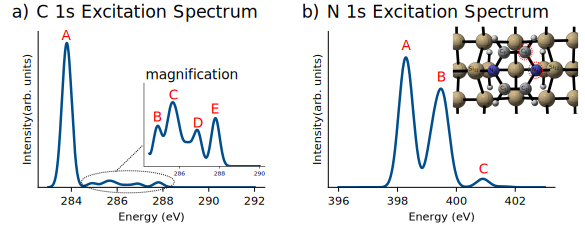
\includegraphics{pyrazine_chemisorbed_c_kedge.pdf}
\caption{Near-edge X-ray absorption spectrum of pyrazine (C$_4$H$_4$N$_2$) chemisorbed on a Si$_{23}$H$_{24}$ cluster model of Si(100) at the a) C K-edge and b) N K-edge computed with OCDFT at the PBE level. All C, N, and H atoms use the cc-pVTZ basis set while the 6-31G basis set is used for the Si atoms of the cluster model. The inset in the C spectrum magnifies the $\sigma^*$ manifold of the spectrum. The pyrazine geometry optimized at the B3LYP/6-31G* level is shown in the inset in the N spectrum, the atoms circled (C$_8$ and N$_4$) are the core holes considered in further discussion of the results in this section.}
\label{fig:chem_pyrazine_nexafs}
\end{figure}

\subsection*{NEXAFS Spectrum of Chemisorbed Pyrazine on Si(100)}
The OCDFT simulated NEXAFS spectrum of pyrazine chemisorbed on the Si(100) surface is shown in Figure \ref{fig:chem_pyrazine_nexafs}. The LIVVOs shown in Figure \ref{fig:chem_pyrazine_livvos} are only those that are directly involved with the adsorbed pyrazine molecule. In total, this system produces 70 LIVVOs however many of these are $\sigma^*_{\rm Si-Si}$ and  $\sigma^*_{\rm Si-H}$ orbitals related to the Si(100) cluster model. When comparing the LIVVOs of the chemisorbed complex to that of free pyrazine, many of the orbitals are remain unchanged except for  three critical differences. First, the most obvious difference is the appearance of the $\sigma^*_{\rm N_3-Si_{11}}$ and $\sigma^*_{\rm N_4-Si_{12}}$ LIVVOs to reflect the covalent bonds formed between the cluster and the para nitrogens on pyrazine. Secondly, the $\pi$ system of the molecule has changed and the LIVVOs reflect that, the $\pi^*$ orbitals are not localized along the N-C bonds, as is the case in free pyrazine, they are now localized along each C=C double bond with clear contributions from the N lone pair electrons. Lastly the $\sigma^*_{\rm Si_{13}-Si_{14}}$ represents the dangling bonds that exist at each open Si site on the dimers. These changes in the character of the LIVVOs gives us some insight into the effect of the cluster on the adsorbate. 

\begin{figure}[b!]
\centering
\includegraphics{pyrazine_chem_livvos.pdf}
\caption{LIVVOs used to analyze particle orbitals in pyrazine (C$_4$H$_4$N$_2$) chemisorbed on a Si$_{23}$H$_{24}$ cluster model of Si(100).}
\label{fig:chem_pyrazine_livvos}
\end{figure}

Since pyrazine maintains two double bonds upon binding on the surface, the NEXAFS spectrum can be expected to maintain the same general spectral pattern of a sharp $\pi^*$ peak and a weaker $\sigma^*$ manifold. The experimental NEXAFS spectrum of chemisorbed pyrazine reports the initial spectral feature at 285.9 attributed to a $\pi^*$ excitation. Our results show an initial excitation at 279.4 eV that is attributed to a $\sigma^*_{\rm Si_{13}-Si_{14}}$, which is the orbital associated with he open Si atoms. The appearance of this state in our calculations is purely an artifact of the cluster model. In reality, pyrazine forms a 1D molecular chain along the surface, leaving few open Si sites on the surface and thus quenching this state. State 2 at 283.8 eV agrees well with the experimental onset feature, is assigned to $\pi^*$ LIVVVOs, and is the sole contribution to Peak A in the spectrum. Considering the core hole at atom C$_8$ State 2 is localized heavily toward the core hole, with 73.4\% of the orbital character attributed to the $\pi^*_{C_7-C_8}$ LIVVO, this is similar to the localization along a single $\pi^*$ bond seen in the gas phase spectrum where the first state had 78.2\% overlap with a single $\pi^*$ LIVVO. The similarity between the LIVVO localization of the $\pi^*$ state in the gas and condensed phases considered here shows that the localization of this $\pi^*$ state is not significantly affected upon adsorption to the surface. Due to this, there is a large difference in intensity at the C K-edge of chemisorbed pyrazine between the $\pi^*$ peak and the $\sigma^*$ manifold, that didn't exist in the spectrum of free pyrazine. The crucial difference here is the interaction and subsequent rehybridization of the pyrazine valence orbitals with the Si cluster. Looking at the particle orbital $\phi^{(2)}_{\rm p}$ it is clear that this initial $\pi^*$ state interacts very little with the Si cluster, meanwhile every other particle orbital has significant contribution from Si cluster orbitals. This can also be seen quantitatively by looking at the LIVVO assignments in Table \ref{tab:chem_pyrazine_states}, for the $\pi^*$ state (State 2), a single VVO constitutes 76\% of the total valence character, in contrast no other state has a single VVO contribution of over 20\%. As a result, the $\sigma^*$ manifold for the C 1s spectrum is orders of magnitude less intense than the $\pi^*$ feature. 



The N 1s spectrum shown in Figure \ref{fig:chem_pyrazine_nexafs}b, does not show the same stark contrast in intensity as the C spectrum. This is due to the fact that the $\pi^*$ orbitals are now localized away from the N atoms upon the formation of the covalent Si-N bonds. In fact, in contrast to all other spectra considered here, the pure $\pi^*$ state (State 10) is the highest in energy at 401.6 eV and has an oscillator strength of zero. Interestingly this is not the only state to provide no intensity to the spectrum. States 6 and 7 also provide no intensity to the spectrum due to their interaction with the cluster, both states have no contributions from LIVVOs that are localized on the pyrazine molecule and their respective particle orbitals in Figure \ref{fig:chem_pyrazine_parts}b ($\phi^{(6)}_{\rm p}$ and $\phi^{(7)}_{\rm p}$) clearly shows no interactions from pyrazine. 

\begin{figure}[t!]
\centering
\includegraphics{n_and_c_chem_particles.pdf}
\caption{Particle orbitals for the core excited states that contribute to the a) carbon and b) nitrogen 1s excitation spectrum of pyrazine (C$_4$H$_4$N$_2$) chemisorbed on a Si$_{23}$H$_{24}$ cluster model of Si(100).}
\label{fig:chem_pyrazine_parts}
\end{figure}

Peak A of the N 1s spectrum has contributions from States 1 and 2, similar to the C 1s spectrum this first state is an artifact of the cluster from the open Si sites. State 2 however is a contribution from the Si-N bond, $\phi^(2)_{\rm p}$ has 39.7\% overlap with the $\sigma^*_{\rm N_4-Si_{12}}$ LIVVO. Peak B has contributions from States 3 and 4 both of which are mixed $\pi^*$/$\sigma^*$ states. Similar to the C 1s spectrum, this ratio favors $\sigma^*$ character due to interaction with the cluster model. The sole contribution to Peak C is a weak transition attributed to the $\pi^*$ orbitals with 5.2\% overlap with $\pi^*_{\rm C_7-C_8}$ and 4.9\% overlap with $\pi^*_{\rm C_1-C_2}$.  

\begin{table}
\centering
\footnotesize
\caption{Calculated (PBE/cc-pVTZ) core excitation energies, oscillator strengths, and LIVVO assignments for the C and N 1s excitation spectrum of pyrazine (C$_4$H$_4$N$_2$) chemisorbed on a Si$_{23}$H$_{24}$ cluster model of Si(100). The LIVVO assignments shown are the two with the highest percentage overlap with the particle orbital. For each calculated transition we report the $\pi^*$/$\sigma^*$ mixing ratio (see text for details) and the spectral feature that this state contributes to (see Figure \ref{fig:chem_pyrazine_nexafs}). }
\begin{tabular}{cccS[]ccc}
\hline
\hline
State & energy (eV) & osc & \rm \centering LIVVO Assignments & $\pi^*/\sigma^*$ Mixing & $t_{\rm p}^{\rm val}$ & Peak Contribution \\
\hline
\multicolumn{7}{c}{\bf C 1s Core Excitations} \\
1 & 279.4 & 0.0002 & 83.8\% $\sigma^*_{\rm Si_{13}-Si_{14}}$ & 1\% $\pi^*$/99\%$\sigma^*$ & 98.2\% & \\
2 & 283.8 & 0.0210& 73.4\% $\pi^*_{\rm C_7-C_8}$ & 86\% $\pi^*$/24\%$\sigma^*$ & 97.0\% & A \\
 & & & 10.5\% $\pi^*_{\rm C_1-C_2}$ & & & \\
 3 & 284.9 & 0.0005 & 11.8\% $\sigma^*_{\rm N_3-Si_{11}}$ & 100\%$\sigma^*$ & 92.2\% & B \\
 & & & 10.1\% $\sigma^*_{\rm N_4-Si_{12}}$ & & & \\
  4 & 285.3 & 0.0002 & 18.5\% $\pi^*_{\rm C_1-C_2}$ & 21\%$\pi^*$/79\%$\sigma^*$ & 92.2\% & C \\
 & & & 13.2\% $\sigma^*_{\rm N_3-Si_{11}}$ & & & \\
  5 & 285.6 & 0.0006 & 9.7\% $\pi^*_{\rm C_1-C_2}$ & 12\%$\pi^*/88\%$\sigma^*$ & 89.5\% & C \\
 & & & 4.0 \% $\sigma^*_{\rm C_8-H_{10}}$ & & & \\
       6 & 285.8 & 0.0005 & 11.4\% $\pi^*_{\rm C_7-C_8}$ & 14\%$\pi^*/86\%$\sigma^*$ & 89.9\% & C \\
 & & & 5.7 \% $\sigma^*_{\rm N_3-Si_{11}}$ & & & \\
   7 & 286.4 & 0.0003& 10.5\% $\sigma^*_{\rm C_8-H_{10}}$ & 100\%$\sigma^*$ & 87.2\% & D\\
 & & & 1.7 \% $\sigma^*_{\rm N_3-Si_{11}}$ & & & \\
    8 & 286.3 & 0.0000 & 2.1\% $\pi^*_{\rm C_7-C_8}$ & 3\%$\pi^*/97\%$\sigma^*$ & 91.0\% & D \\
 & & & 0.6\% $\pi^*_{\rm C_7-C_8}$ & & & \\
   9 & 286.9 & 0.0005 & 13.3\% $\sigma^*_{\rm C_8-H_{10}}$ & 2\%$\pi^*/98\%$\sigma^*$ & 83.9\% & D \\
 & & & 1.6\% $\sigma^*_{\rm C_7-H_9}$ & & & \\
    10 & 287.8 & 0.0007 & 12.0\% $\sigma^*_{\rm N_4-Si_{12}}$ & 4\%$\pi^*/96\%$\sigma^*$ & 89.9\% & E \\
 & & & 3.7 \% $\sigma^*_{\rm N_4-C_8}$ & & & \\
 \multicolumn{7}{c}{\bf N 1s Core Excitations} \\
     1 & 398.2 & 0.0026 & 85.1\% $\sigma^*_{\rm Si_{13}-Si_{14}}$ & 1\%$\pi^*/99\%$\sigma^*$ & 98.7\% & A \\
 & & & 1.3 \% $\sigma^*_{\rm N_4-Si_{12}}$ & & & \\
       2 & 398.4 & 0.0016 & 39.7\% $\sigma^*_{\rm N_4-Si_{12}}$ & 2\%$\pi^*/98\%$\sigma^*$ & 93.3\% & A \\
 & & & 2.1 \% $\sigma^*_{\rm N_4-C_8}$ & & & \\
        3 & 399.2 & 0.0010 & 12.3\% $\sigma^*_{\rm N_3-Si_{11}}$ & 15\%$\pi^*/85\%$\sigma^*$ & 92.8\% & B \\
 & & & 7.6 \% $\pi^*_{\rm C_7-C_8}$ & & & \\
         4 & 399.5 & 0.0010 & 11.0\% $\pi^*_{\rm C_7-C_8}$ & 22\%$\pi^*/78\%$\sigma^*$ & 92.2\% & B \\
 & & & 6.3 \% $\sigma^*_{\rm N_3-Si_{11}}$ & & & \\
           5 & 399.6 & 0.0005 & 9.9\% $\sigma^*_{\rm N_3-Si_{11}}$ & 12\%$\pi^*/88\%$\sigma^*$ & 89.9\% & B \\
 & & & 5.5 \% $\pi^*_{\rm C_7-C_8}$ & & & \\
            6 & 399.7 & 0.0003 & 5.6\% $\sigma^*_{\rm N_3-Si_{11}}$ & 5\%$\pi^*/95\%$\sigma^*$ & 89.9\% & B \\
 & & & 2.3 \% $\pi^*_{\rm C_7-C_8}$ & & & \\
             7 & 400.2 & 0.0000 & N/A & 100\%$\sigma^*$ & 91.3\% &  \\
          8 & 400.5 & 0.0000 & N/A & 100\%$\sigma^*$ & 91.3\% & \\
                       9 & 400.9 & 0.0003 & 5.2\% $\pi^*_{\rm C_7-C_8}$ & 12\%$\pi^*/88\%$\sigma^*$ & 87.8\% & C \\
 & & & 4.9 \% $\pi^*_{\rm C_1-C_2}$ & & & \\
      10 & 401.6 & 0.0000 & 44.2\% $\pi^*_{\rm C_1-C_2}$ & 87\%$\pi^*/13\%$\sigma^*$ & 95.7\% & \\
 & & & 38.9 \% $\pi^*_{\rm C_7-C_8}$ & & & \\
\hline
\end{tabular}
\label{tab:chem_pyrazine_states}
\end{table}
%To help understand what happens to the NEXAFS spectra of the molecules upon chemisorption it is important to first consider the core-excitations in gas-phase acetylene, ethylene, and benzene. Table \ref{tab:gas_phase_tab} shows the calculated core-excitation energies, oscillator strengths, and dominant atomic transitions of all three molecules in the gas-phase. Due to the presence symmetry equivalent carbon atoms in each molecule, we perform broken symmetry OCDFT calculations in order to obtain a solution with a localized core hole. When compared to the experimental peak positions, OCDFT has a mean average error of 0.5 eV across the 9 transitions considered in these three molecules, representing excellent agreement with experiment. This degree of accuracy is commensurate with previous OCDFT studies on gas-phase organic molecules.\cite{derricotte_simulation_2015,verma_predicting_2016} Our consideration of the atomic contributions to the electronic dipole moment along with the OCDFT particle orbitals help facilitate the assignments shown in Table \ref{tab:gas_phase_tab}. For more information on the gas-phase particle orbitals and simulated spectra for all three molecules in the gas-phase we refer the reader to the Supporting Information. 

%\begin{table}
%\footnotesize
%\caption{Calculated core-excitation energies, oscillator strengths, and dominant atomic transitions ($|\mathrm{A}_{l_\mathrm{A}} \rightarrow \mathrm{B}_{l_\mathrm{B}} |_{\rm max}$) for acetylene, ethylene, and benzene calculated with OCDFT at the B3LYP/cc-pVTZ level of theory. Spectra were simulated by calculating 10 unique carbon core-excitations for each carbon atom in the molecule. Only transitions shown here are non-redundant transitions with a relative oscillator strength of 0.1 or higher}
%\begin{tabular}{cccc}
%\hline
%\hline
%exp. (eV)[\citenum{hitchcock_carbon_1977}] & OCDFT (eV) & f$_{\rm osc}$ & $|\mathrm{A}_{l_\mathrm{A}} \rightarrow \mathrm{B}_{l_\mathrm{B}} |_{\rm max}$\\
%\hline
%\multicolumn{4}{c}{\bf Acetylene} \\
%285.9 & 285.6 & 1.00 & C$_{\rm s}$ $\rightarrow$ C$_{\rm p}$ \\
%288.1 & 288.6 & 0.37 & C$_{\rm s}$ $\rightarrow$ H$_{\rm s}$ \\
%290.1 & 290.9 & 0.13 & C$_{\rm s}$ $\rightarrow$ H$_{\rm s}$ \\
%\multicolumn{4}{c}{\bf Ethylene} \\
%284.7 & 284.6 & 1.00 & C$_{\rm s}$ $\rightarrow$ C$_{\rm p}$ \\
%\multirow{2}{*}{287.4} & 287.8 & 0.21 & C$_{\rm s}$ $\rightarrow$ H$_{\rm s}$ \\
%& 288.2 & 0.57 & C$_{\rm s}$ $\rightarrow$ H$_{\rm s}$ \\
%290.1 & 290.4 & 0.19 & C$_{\rm s}$ $\rightarrow$ H$_{\rm s}$ \\
%\multicolumn{4}{c}{\bf Benzene} \\
%285.2 & 285.2 & 1.00 & C$_{\rm s}$ $\rightarrow$ C$_{\rm p}$ \\
%\multirow{2}{*}{287.2} & 287.8 & 0.28 & C$_{\rm s}$ $\rightarrow$ H$_{\rm s}$ \\
%& 288.2 & 0.43 & C$_{\rm s}$ $\rightarrow$ H$_{\rm s}$ \\
%289.0 & 289.4 & 0.84 & C$_{\rm s}$ $\rightarrow$ C$_{\rm p}$ \\
%\hline
%\hline
%\end{tabular}
%\label{tab:gas_phase_tab}
%\end{table}

%\begin{table}
%\begin{tabular}{cccl}
%\hline
%\hline
%State &Energy (eV) & $f_{osc}$ & LIVVO Assignment \\
%\hline
%1 & 284.1 &  0.0019 & 85.9\% $\sigma^*_{\rm Si-N-C-Si}$ \\
%2 & 286.0 &  0.0189 & 77.3\% $\pi^*_{\rm C_1-C_2}$\\
%& & & 8.9\% $\pi^*_{\rm C_3-C_4}$ \\
%3 &287.4 &  0.0007 & 10.1\% $\sigma^*_{\rm N_1-Si}$ \\
%& & & 10.1\% $\sigma^*_{\rm N_2-Si}$ \\
%4 & 288.4 &  0.0009 & 8.5\% $\sigma^*_{\rm C_3-C_4}$\\
%& & & 7.0\% $\pi^*_{\rm C_3-C_4}$ \\
%5 & 287.8 &  0.0000 & 13.8\% $\pi^*_{\rm C_3-C_4}$ \\
%& & & 12.3\% $\sigma^*_{\rm N_2-Si}$ \\
 %\hline
 %\end{tabular}
%\end{table}

%\subsection*{Acetylene and Ethylene}
%The OCDFT calculated C K-edge of chemisorbed acetylene shown in Figure \ref{fig:all}a is characterized by three distinct spectral features at 284.3, 285.8, and 287.5 eV. The lowest energy peak feature at 284.3 is classified as $\pi^*_{\rm C-C}$ due to the $\pi^*$ character of the particle orbital (shown in Figure \ref{fig:chem_parts}) and that the dominant atomic transitions (shown in Table \ref{tab:ace_eth_tab}) are from C$_{\rm s}$ $\rightarrow$  C$_{\rm p}$. Similarly we classified the two higher energy peaks as $\sigma^*_{\rm C-Si}$ and $\sigma^*_{\rm C-H}$ due to their $\sigma^*$ particle orbital character and the dominance of C$_{\rm s}$ $\rightarrow$  Si$_{\rm p}$ and C$_{\rm s}$ $\rightarrow$  H$_{\rm s}$ contributions. The spectral features of the calculated spectrum agree well with the experimental peak positions of 284.7, 286.0, and 287.6 eV and the assignments made here are also in accordance with the experimental assignments.\cite{matsui_adsorption_2000} 
\begin{comment}
\begin{table}[!b]
\footnotesize
\caption{Calculated chemisorbed acetylene and ethylene OCDFT(B3LYP) carbon core excitation energies using the cc-pVTZ basis set for C and H atoms and the 6-31G basis set for Si atoms. The most dominant atomic transition ($|\mathrm{A}_{l_\mathrm{A}} \rightarrow \mathrm{B}_{l_\mathrm{B}}|_{\rm max}$) for each excitation is shown as well as the assignments from the experimental study. The transitions shown have a relative oscillator strength of 0.1 or higher, for a full table of all calculated transitions, we refer the reader to the supplementary material. }
\begin{tabular}{cccc}
\hline
\hline
Energy (eV) & $f_{\rm osc}$ & $|\mathrm{A}_{l_\mathrm{A}} \rightarrow \mathrm{B}_{l_\mathrm{B}}|_{\rm max}$ & exp. [\citenum{matsui_adsorption_2000}]\\
\hline
\multicolumn{4}{c}{\bf Acetylene on Si(100)} \\
284.29 & 1.00 & C$_{\rm s}$ $\rightarrow$ C$_{\rm p}$ &\multirow{2}{*}{$\pi^*_{\rm C-C}$(284.7)}\\
284.29 & 1.00 & C$_{\rm s}$ $\rightarrow$ C$_{\rm p}$ \\
285.82 & 0.32 & C$_{\rm s}$ $\rightarrow$ Si$_{\rm p}$ &\multirow{2}{*}{$\sigma^*_{\rm Si-C}$(286.0)}\\
285.82 & 0.32 & C$_{\rm s}$ $\rightarrow$ Si$_{\rm p}$ \\
287.49 & 0.22 & C$_{\rm s}$ $\rightarrow$ H$_{\rm s}$ &\multirow{4}{*}{$\sigma^*_{\rm H-C}$(287.6)}\\
287.49 & 0.22 & C$_{\rm s}$ $\rightarrow$ H$_{\rm s}$ \\
287.76 & 0.12 & C$_{\rm s}$ $\rightarrow$ H$_{\rm s}$ \\
287.76 & 0.12 & C$_{\rm s}$ $\rightarrow$ H$_{\rm s}$ \\
\multicolumn{4}{c}{\bf Ethylene on Si(100)} \\
285.82 & 1.00 & C$_{\rm s}$ $\rightarrow$ Si$_{\rm p}$ & \multirow{4}{*}{$\sigma^*_{\rm Si-C}$(285.6)}\\
285.82 & 1.00 & C$_{\rm s}$ $\rightarrow$ Si$_{\rm p}$ \\
286.41 & 0.14 & C$_{\rm s}$ $\rightarrow$ Si$_{\rm s}$ \\
286.43 & 0.14 & C$_{\rm s}$ $\rightarrow$ Si$_{\rm s}$ \\
286.84 & 0.20 & C$_{\rm s}$ $\rightarrow$ H$_{\rm s}$ & \multirow{4}{*}{$\sigma^*_{\rm H-C}$(287.0)}\\
286.86 & 0.20 & C$_{\rm s}$ $\rightarrow$ H$_{\rm s}$ \\
286.88 & 0.47 & C$_{\rm s}$ $\rightarrow$ H$_{\rm s}$ \\
286.90 & 0.47 & C$_{\rm s}$ $\rightarrow$ H$_{\rm s}$ \\
287.60 & 0.50 & C$_{\rm s}$ $\rightarrow$ H$_{\rm s}$ & \multirow{8}{*}{$\pi^*_{\rm H-C}$(288.1)} \\
287.62 & 0.34 & C$_{\rm s}$ $\rightarrow$ H$_{\rm s}$ \\
287.81 & 0.48 & C$_{\rm s}$ $\rightarrow$ H$_{\rm s}$ \\
287.85 & 0.78 & C$_{\rm s}$ $\rightarrow$ H$_{\rm s}$ \\
287.89 & 0.81 & C$_{\rm s}$ $\rightarrow$ H$_{\rm s}$ \\
287.94 & 0.88 & C$_{\rm s}$ $\rightarrow$ H$_{\rm s}$ \\
288.14 & 0.23 & C$_{\rm s}$ $\rightarrow$ H$_{\rm s}$ \\
288.30 & 0.23 & C$_{\rm s}$ $\rightarrow$ H$_{\rm s}$ \\
\hline
\end{tabular}
\label{tab:ace_eth_tab}
\end{table}
\end{comment}

%Comparison of the $\pi^*_{\rm C-C}$ peak of gas-phase acetylene and the chemisorbed species shows that the latter exhibits a significant redshift of 1.2 eV. Work from Besley and Noble\cite{besley_time-dependent_2007} attributes this shift solely to the lengthening of the C$-$C bond upon adsorption. However it is unclear whether or not this bond elongation (about 0.15\AA) is the sole factor contributing to the redshift or if other considerations play a more significant role. To fully understand the cause of this shift upon absorption, we conducted a study on five different systems shown in Table \ref{tab:const_data}, calculating the C$_{1s}$ $\rightarrow$ $\pi^*_{\rm C-C}$ transition in each case. When the C$-$C bond is stretched by 0.15~\AA~the excitation energy blueshifts by 0.1 eV compared to the same transition in the optimized structure. This suggests that the cause of this shift is not solely a byproduct of the stretching of the C$-$C bond. When including the bend of the C$-$H bonds, there is a more significant shift of 0.8 eV, this accounts for a large portion of the redshift upon adsorption but not the entire shift. It is only when we include the Si$-$C bonds in the Si$_2$H$_4$ model system that we can reproduce the full shift. So the lengthening of the C$-$C bond is not the only factor that contributes to the redshift of the $\pi^*_{\rm C-C}$ peak chemisorbed acetylene, it is also the geometric alterations of the C$-$H bonds and the formation of the Si$-$C bonds that account for a large portion of this shift upon adsorption. 

\begin{comment}
\begin{table*}
\footnotesize
\caption{Calculated C$_{1s}$ $\rightarrow$ $\pi^*_{\rm C-C}$ excitation energy, C$-$C bond length (r$_{C-C}$), C$-$C$-$H dihedral angle ($\theta_{\rm C-C-H}$), and number of Si-C bonds in 5 different acetylene systems. The gas-phase and full chemisorbed structures (on Si$_9$H$_{12}$) are optimized at the B3LYP/6-31G* level of theory, all other structures are derived from these optimized structures.} 
\begin{tabular}{cccccc}
\hline
\hline
\multicolumn{2}{c}{System} & r$_{\rm C-C}$ (\AA)& $\theta_{\rm C-C-H}$ & Si-C bonds & excitation energy (eV)\\
\hline
\vspace{0.04cm}\\
\raisebox{-0.7cm}[0.5cm][0.5cm]{\includegraphics[width=0.1\textwidth, height=0.1\textwidth]{c2h2_gas.pdf}} & gas-phase & 1.21 & 180.0$^{\circ}$ & 0 & 285.5 \\
\raisebox{-0.7cm}[0.5cm][0.5cm]{\includegraphics[width=0.1\textwidth, height=0.1\textwidth]{c2h2_stretch.pdf}} & stretch & 1.36 & 180.0$^{\circ}$ & 0 & 285.6 \\
\raisebox{-0.7cm}[0.5cm][0.5cm]{\includegraphics[width=0.1\textwidth, height=0.1\textwidth]{c2h2_bent.pdf}} & bent & 1.36 & 123.5$^{\circ}$ & 0 & 284.7 \\
\raisebox{-0.7cm}[0.5cm][0.5cm]{\includegraphics[width=0.1\textwidth, height=0.1\textwidth]{c2h2_onsi2.pdf}} & on Si$_2$H$_4$ & 1.36 & 123.5$^{\circ}$ & 2 & 284.2 \\
\raisebox{-0.85cm}[0.5cm][0.5cm]{\includegraphics[width=0.1\textwidth, height=0.1\textwidth]{c2h2_full.pdf}} & on Si$_9$H$_{12}$ & 1.36 & 123.5$^{\circ}$ & 2 & 284.2\vspace{0.1cm}\\
\hline
\hline
\end{tabular}
\label{tab:const_data}
\end{table*}

\end{comment}

%the most intense transition corresponds to the C$_{1s}$ $\rightarrow$ $\pi^*_{\rm C-C}$. This transition is predicted to occur at 284.3, which is close to the predicted experimental value of 284.7. This error of about 0.5 eV is commensurate with the error of OCDFT when calculating core excitations in gas-phase organic molecules, it is encouraging to see that energies for chemisorbed organic molecules can be represented with the same level of accuracy. Two spectral features at higher energy are predicted at 285.8 and 287.5 eV, these correspond to $\sigma^*_{\rm C-Si}$ and $\sigma^*_{\rm C-H}$ transitions respectively. For the C$_{1s}$ $\rightarrow$ $\pi^*_{\rm C-C}$ transition, the most dominant atomic transition is from C$_{\rm s}$ $\rightarrow$ C$_{\rm p}$. Analysis of the peak at 285.8 eV shows that the most dominant atomic contribution is from C$_{\rm s}$ $\rightarrow$ Si$_{\rm s}$, this is consistent with the experimental assignment of this transition as C$_{1s}$ $\rightarrow$ $\sigma^*_{\rm C-Si}$. For the peak at 287.5 eV, the most dominant atomic contributions to this transition is C$_s$ $\rightarrow$ H$_s$ which is again consistent with the experimental assignment of this peak as C$_{\rm 1s}$ $\rightarrow$ $\sigma^*_{\rm C-H}$. It should be noted that there are other transitions in this region that have C$_{\rm s}$ $\rightarrow$ Si$_{\rm s}$ and C$_{\rm s}$ $\rightarrow$ Si$_{\rm p}$ character yet their dipole contributions are relatively negligible. The particle orbitals plotted in the top panel of Figure \ref{fig:all}a along with the atomic dipole decomposition in the bottom panel of Figure \ref{fig:all}a provide a clear and unambiguous interpretation of each spectral feature. Table \ref{tab:c2h2_table} shows the most significant calculated transitions, for full Mulliken analysis of all of our calculated transitions, we direct the reader to the supplementary material.


%The experimental spectrum of acetylene detected three transitions below the ionization potential at 284.7, 286.0, and 287.6 eV assigned to $\pi^*_{\rm C-C}$ , $\sigma^*_{\rm C-Si}$, and $\sigma^*_{\rm C-H}$ respectively. The calculated spectrum of C$_2$H$_2$ chemisorbed on the Si$_9$H$_{12}$ model of the Si(100) surface is reported in Figure \ref{fig:c2h2_atomic}. Our DFT optimized structure predicts a C$-$C bond length of 1.36\AA and a Si$-$Si bond length of 2.37\AA. Experimentally determined bonds have a high degree of uncertainty, with the C$-$C bond length estimated in a range of 1.32 -- 1.37\AA and the Si$-$Si dimer bond estimated at 2.44 $\pm$ 0.58\AA, our optimized structures are consistent with these experimental estimates.

%\begin{figure*}
%\centering
%\includegraphics[scale=0.8]{all_spectra.pdf}
%\caption{Near-edge X-ray absorption spectrum of a) acetylene, b) ethylene, c) benzene(butterfly), and d) benzene(tilted) adsorbed on Si(100). Computed with X2C-OCDFT at the B3LYP/un-aug-cc-pVDZ level of theory. Spectra were simulated by calculating 10 unique carbon core-excitations for each carbon atom. Transitions are convoluted with gaussians of FWHM=0.5 eV. A restricted excitation window energy cutoff of 20 eh was used to target C K-edge. Experimental peak positions are shown as dashed vertical lines for comparison.}
%\label{fig:Acetylene_spectrum}
%\end{figure*}

%\begin{figure}[h!]
%\centering
%\includegraphics[scale=1.0]{acetylene_spec_and_atomic_with_orbs.pdf}
%\caption{a) Carbon K-edge spectrum of acetylene calculated using OCDFT(B3LYP). All carbon (silver) and hydrogen (white) atoms are represented by the cc-pvtz basis set, while all silicon (brown) atoms are represented by the 6-31G basis set. The orbitals shown are the partical orbitals ($\phi_{\rm p}$) corresponding to the most intense contribution to the specified peak feature. b) Atomic orbital contributions to the total electric dipole for each C core excitation in acetylene. Each transition is color coded based on the most dominant atomic contribution to the dipole for that transition where red represents carbon p orbitals, green represents hydrogen s orbitals, and blue represents silicon s and p orbitals.}
%\label{fig:c2h2_atomic}
%\end{figure}
%\begin{table}
%\footnotesize
%\caption{Calculated acetylene OCDFT(B3LYP) carbon core excitation energies using the cc-pvtz basis set for C and H atoms and the 6-31G basis set for Si atoms. The most dominant atomic transition ($|\mathrm{A}_{l_\mathrm{A}} \rightarrow \mathrm{B}_{l_\mathrm{B}}|_{\rm max}$) for each excitation is shown as well as the assignments from the experimental study. Only transitions shown are those with a relative oscillator strength of 0.1 or higher, for a full table of all calculated transitions, we refer the reader to the supplementary material. }
%\begin{tabular}{cccc}
%\hline
%\hline
%Energy (eV) & $f_{\rm osc}$ & $|\mathrm{A}_{l_\mathrm{A}} \rightarrow \mathrm{B}_{l_\mathrm{B}} |_{\rm max}$ & exp.[\citenum{matsui_adsorption_2000}]\\
%\hline
%284.29 & 1.00000 & C$_{\rm s}$ $\rightarrow$ C$_{\rm p}$ &\multirow{2}{*}{$\pi^*_{\rm C-C}$(284.7)}\\
%284.29 & 0.99749 & C$_{\rm s}$ $\rightarrow$ C$_{\rm p}$ \\
%285.82 & 0.32435 & C$_{\rm s}$ $\rightarrow$ Si$_{\rm p}$ &\multirow{2}{*}{$\sigma^*_{\rm Si-C}$(286.0)}\\
%285.82 & 0.32117 & C$_{\rm s}$ $\rightarrow$ Si$_{\rm p}$ \\
%287.49 & 0.21845 & C$_{\rm s}$ $\rightarrow$ H$_{\rm s}$ &\multirow{4}{*}{$\sigma^*_{\rm H-C}$(287.6)}\\
%287.49 & 0.21993 & C$_{\rm s}$ $\rightarrow$ H$_{\rm s}$ \\
%287.76 & 0.12117 & C$_{\rm s}$ $\rightarrow$ H$_{\rm s}$ \\
%287.76 & 0.11782 & C$_{\rm s}$ $\rightarrow$ H$_{\rm s}$ \\
%\hline
%\end{tabular}
%\label{tab:c2h2_table}
%\end{table}



%\begin{figure}[h!]
%\centering
%\includegraphics[scale=0.4]{acetylene_atomic_plot.pdf}
%\caption{Atomic orbital contributions to the total electric dipole for each C core excitation in acetylene. Each transition is color coded based on the most dominant atomic contribution to the dipole for that transition where red represents carbon p orbitals, green represents hydrogen s orbitals, and blue represents silicon s and p orbitals.}
%\label{fig:c2h2_atomic}
%\end{figure}

%\begin{figure}[h!]
%\centering
%\includegraphics[scale=0.4]{acetylene_adsorbed.pdf}
%\caption{C K-edge spectrum of acetylene calculated using OCDFT(B3LYP). All carbon (silver) and hydrogen (white) atoms are represented by the cc-pvtz basis set, while all silicon (brown) atoms are represented by the 6-31G basis set.}
%\label{fig:c2h2_atomic}
%\end{figure}

%\begin{figure}
%\includegraphics[scale=0.4]{c2h2_gas_spectrum.pdf}
%\caption{Near-edge X-ray absorption spectrum gas-phase acetylene. Computed with X2C-OCDFT at the B3LYP/un-aug-cc-pVDZ level of theory. Spectrum was simulated by calculating 10 unique carbon core-excitations for each carbon atom. Transitions are convoluted with gaussians of FWHM=0.5 eV.}
%\label{fig:acetylene_gas}
%\end{figure}

%Calculations of the gas-phase spectrum of acetylene (see Figure \ref{gas_phase}a) predict an excitation energy of 285.5 eV for the $\pi^*_{\rm C-C}$ transition. Compared to this, the $\pi^*_{\rm C-C}$ peak in chemisorbed acetylene exhibits a significant redshift of 1.2 eV. Work from Besley and Noble attributes this shift solely to the lengthening of the C$-$C bond upon adsorption, our optimized structures show that there is a lengthening of the C$-$C bond of about 0.15\AA~in the chemisorbed complex. But in order to understand the shift of this peak feature upon absorption, we conducted a study on five different systems (shown in Table \ref{tab:const_data}): 1) The equilibrium gas-phase acetylene molecule with a bond length of 1.21\AA~2) a linear acetylene molecule with the bond length stretched to 1.36\AA~ to mimic the C$-$C bond length of chemisorbed acetylene. 3) a bent acetylene molecule that has the stretched C$-$C bond length as well as the C$-$C$-$H angle of 123.5$^{\circ}$ to mimic all of the local geometrical changes that acetylene undergoes upon adsorption and 4) a miniature Si$_2$H$_4$ model in order to include the bonding to the Si$-$Si dimer. 5) Acetylene adsorbed to the full Si$_9$H$_{12}$ single dimer cluster. The C$_{1s}$ $\rightarrow$ $\pi^*_{\rm C-C}$ transition was calculated in each case and is reported in Table \ref{tab:const_data}, when stretching the bond by 0.15\AA~ this transition does not shift significantly. So clearly, the cause of this shift is not solely a byproduct of the stretching of the C$-$C bond. When including the bend of the C$-$H bonds, there is a more significant shift of 0.8 eV, this accounts for a large portion of the redshift upon adsorption but not the entire shift. It is only when we include the Si$-$C bonds in the Si$_2$H$_4$ model system that we can reproduce the full shift. So the true explanation for the cause of this shift is somewhere between the theoretical and experimental explanation. Matsui is correct that the charge transfer that occurs between the Si dimer and the acetylene molecule upon adsorption plays a role in this shift, however according to our calculations it only accounts for 0.4 eV of this shift. Besley and Noble were on the right track to assume that this shift is a by product of a local geometric change, considering how localized the $\pi^*$ orbital is to the adsorbate, this makes sense. But it is not solely the lengthening of the C$-$C bond, it is also the geometric alterations of the C$-$H bonds that account for a large portion of this shift upon adsorption. 

%\begin{figure*}
%\centering
%\includegraphics{acetylene_ethylene.pdf}
%\caption{a) Carbon K-edge spectrum of acetylene and ethylene on a single dimer silicon surface calculated using OCDFT(B3LYP). All carbon (silver) and hydrogen (white) atoms are represented by the cc-pVTZ basis set, while all silicon (brown) atoms are represented by the 6-31G basis set. b) Atomic orbital contributions to the total electric dipole for each C core excitation in ethylene. Each transition is color coded based on the most dominant atomic contribution to the dipole for that transition where yellow represents transitions to carbon p orbitals, light blue represents transitions to hydrogen s orbitals, and red represents transitions to silicon s and p orbitals.}
%\label{fig:all}
%\end{figure*}

%The $\sigma^*_{\rm C-H}$ transition is shifted by roughly 1.0 eV upon adsorption, with the oscillator strength being slightly quenched. This transition has an absolute oscillator strength of 0.0030 in the gas-phase which drops to 0.0021 upon adsorption. This quenching is a result of the electron density of the particle orbital being spread out across the atoms of the Si cluster model. This observation is consistent with previous studies of chemisorbed organics that show the Rydberg states to be less prominent after adsorption.

%\begin{figure}[b!]
%\includegraphics[scale=0.5]{constrained_sys.pdf}
%\caption{Constrained structures used to study the origin of the $\pi^*$ shift in chemisorbed C$_2$H$_2$, the ``bent'' structure was taken from the optimized chemisorbed structure without considering the atoms of the Si cluster model. The ``stretch'' structure is simply the optimized gas-phase acetylene structure with the C$-$C bond length stretched to match the chemisorbed bond length.}
%\label{fig:constrained_sys}
%\end{figure}

%\subsubsection{Relaxed Surface Scan: Acetylene}
%In order to further study the changes in the spectrum upon adsorption, we performed a full geometry relaxed surface scan of the process. The scan was started with the acetylene molecule and the Si-Si dimer separated by 4.0 \AA, the calculated C K-edge spectrum for this case is shown in Figure \ref{fig:c2h2_surf:scan}a, for the sake of comparison, we have also calculated the spectrum with the Si-cluster removed. Comparison of the two spectra show that the low-energy $\pi^*$ peak is largely unaffected by the presence of the Si cluster. The higher energy states are affected by interactions with the Si cluster and are largely shifted to lower energy and are much less intense than in the case of the geometry in the gas-phase. 

%\begin{figure}
%\includegraphics[scale=2.4]{c2h2_surf_scan.pdf}
%\caption{NEXAFS spectra of acetylene computed at three different snapshots from a geometry relaxed surface scan performed at the B3LYP-D3/6-31G* level of theory. The acetylene/Si-Si dimer distance in each geometry is a) 4.0 \AA, b) 2.7 \AA, and c) 1.9 \AA. The structures in d-f correspond to the acetylene structures from a-c with the Si cluster removed. All spectra were computed with OCDFT at the B3LYP/aug-cc-pvtz level of theory using 10 core excited states from each carbon atom.}
%\label{fig:c2h2_surf:scan}
%\end{figure}

%The second snapshot we consider from the relaxed surface scan has the acetylene molecule separated from the cluster dimer by 2.7 \AA~ at this point, interactions with the Si cluster are causing the hydrogens to bend upward, breaking the 180$^{\circ}$ dihedral angle of the adsorbate. This causes a dramatic change in the $\pi$ system of acetylene, the bending of the hydrogens lifts the degeneracy of the two $\pi^*$-orbitals. This is reflected in the NEXAFS spectrum with two distinct $\pi^*$ peaks, one $\pi^*$ orbital lies perpendicular to the C$-$H bond axis and is unaffected by this bending of the structure. However, the other $\pi^*$ orbital now lies along the C$-$H bond axis, this shifts the transition to lower energy as a result. This splitting is present in the spectrum with the Si cluster (Figure \ref{fig:c2h2_surf:scan}b) or without the Si cluster present (Figure \ref{fig:c2h2_surf:scan}e). The magnitude of the peak splitting is roughly 2.0 eV in both cases and the only major differences in the spectrum are seen in the higher energy Rydberg region. The spectrum in Figure \ref{fig:c2h2_surf:scan}e shows that only considering these geometric changes results in a much more pronounced Rydberg region, however when considering the Si cluster interaction in Figure \ref{fig:c2h2_surf:scan}b these transitions are diluted completely by interactions with the cluster model. 

%Figure \ref{fig:c2h2_surf:scan}c shows the NEXAFS spectrum of the chemisorbed complex, the final snapshot in the relaxed surface scan. Upon chemisorption, acetylene no longer has two vacant $\pi^*$ orbitals, thus the spectrum only has one pronounced $\pi^*$ peak. Figure \ref{fig:c2h2_surf:scan}f shows the spectrum of the chemisorbed geometry without the Si-cluster present, the spectrum shows that the $\pi^*$ splitting is still present and has actually increased in magnitude. This means that further bending of the hydrogens increases the $\pi^*$ splitting.  The highest energy peak is still present in the spectrum and a new spectral feature appears between them at about 285 eV, this is consistent with our assignment of this peak feature as a $\sigma_{\rm Si-C}$, since it is only present in the chemisorbed structure it must be a result of bonding interactions with the Si$-$Si dimer.  

%\subsection*{Ethylene on Si(100)}

%For ethylene, the experimental NEXAFS spectrum also contains four unique spectral features at 285.6, 287.0, 288.1, and 291.0 eV that were attributed to $\sigma^*_{\rm C-Si}$, $\pi^*_{\rm C-H_2}$,  $\sigma^*_{\rm C-H_2}$, $\sigma^*_{\rm C-C}$. \cite{matsui_adsorption_1998,matsui_adsorption_2000} The ethylene molecule undergoes a similar cycloaddition at the Si surface as acetylene which causes a reduction of the C-C double bond to a single bond, effectively eliminating the $\pi^*_{\rm C-C}$ transition that occurs in the gas-phase. The $\pi^*_{\rm C-H_2}$ and $\sigma^*_{\rm C-H_2}$ states exhibit a more modest $-$0.6 eV shift upon adsorption, slightly lower than the shift observed in acetylene. Similar to the acetylene K-edge, the $\sigma^*_{\rm C-C}$ transition is heavily effected by adsorption, exhibiting a 10.0 eV shift compared to the gas-phase spectrum. The $\sigma^*_{\rm C-C}$ shape resonances are known to have an empirical relationship on the C$-$C bond length, this is often used to extract experimental bond lengths from NEXAFS spectra, however this is a controversial practice and is still a hotly debated topic in the literature. \cite{kempgens_reappraisal_1997,piancastelli_neverending_1999,kempgens_correct_1999,gainar_nexafs_2015} 

%The OCDFT C K-edge spectrum of chemisorbed ethylene (see Figure 2b) shows three features at 285.8, 286.9, and 287.9 eV. Upon adsorption, ethylene loses a vacant $\pi^*_{\rm C-C}$ orbital, effectively eliminating the most prominent feature of the gas-phase spectrum at 284.7 eV. The first two peaks of the chemisorbed spectrum are of $\sigma^*$ character with the lower energy peak being dominated by atomic transitions of C$_{\rm s}$ $\rightarrow$ Si$_{\rm p}$ while the higher energy peak is a result of  C$_{\rm s}$ $\rightarrow$ H$_{\rm s}$ atomic transitions.

%There is currently discrepency among the literature regarding the classification of the first two peaks in the spectrum at 285.6 and 287.0 eV. Matsui and coworkers\cite{matsui_adsorption_2000} classify these features as  $\sigma^*_{\rm C-Si}$, and $\pi^*_{\rm C-H}$. In 2003, Hennies et al. performed experiments using a single domain crystal, ensuring that the surface was populated with adjacent dimers. They classified these features as  $\pi^*_{\rm C-Si}$ and $\pi^*_{\rm C-H}$. A 2007 TDDFT study done by Besley and Noble classified these features as $\sigma^*_{\rm C-Si}$ and $\sigma^*_{\rm C-H}$. Figure \ref{fig:all} shows the atomic contributions to the spectrum, the largest atomic dipole contribution to the first peak is C$_s$ $\rightarrow$ Si$_s$ and C$_s$ $\rightarrow$ H$_s$ for the second peak which is consistent with previous assignments of this transition. Inspection of the particle orbitals shown in Figure \ref{fig:chem_parts}, reveals that these transitions are both $\sigma^*$. These analyses together are consistent with the Besley and Noble classification of the states.

%\begin{figure}
%\centering
%\includegraphics{chemisorbed_particles_ace_ethyl.png}
%\caption{Particle orbitals ($\phi_{\rm p}$) from the Near-edge X-ray absorption spectra for chemisorbed acetylene and ethylene calculated with OCDFT at the B3LYP/cc-pVTZ level of theory.}
%\label{fig:chem_parts}
%\end{figure}
 
%The experimental spectrum of ethylene detects three unique spectral features below the ionization potential at 285.6, 287.0, and 288.1 eV assigned to core transtions to  $\pi^*_{\rm C-Si}$, $\pi^*_{\rm C-H}$, and $\sigma^*_{\rm C-H}$ repectively. Our calculated spectrum of C$_2$H$_4$ on the Si$_9$H$_{12}$ cluster model of Si(100) is shown in Figure \ref{fig:all} and predicts these peak features to occur at 285.8, 286.9, and 287.9 eV respectively, representing phenomenal agreement with the experimental spectrum.  

%\begin{figure}[t!]
%\centering
%\includegraphics[scale=1.0]{ethylene_spec_and_atomic_with_orbs.pdf}
%\caption{a) Carbon K-edge spectrum of ethylene calculated using OCDFT(B3LYP). All carbon (silver) and hydrogen (white) atoms are represented by the cc-pvtz basis set, while all silicon (brown) atoms are represented by the 6-31G basis set. b) Atomic orbital contributions to the total electric dipole for each C core excitation in ethylene. Each transition is color coded based on the most dominant atomic contribution to the dipole for that transition where red represents carbon p orbitals, green represents hydrogen s orbitals, and blue represents silicon s and p orbitals.}
%\label{fig:c2h4_atomic}
%\end{figure}
%\begin{figure}
%\includegraphics[scale=0.7]{ace_orbs.pdf}
%\end{figure}

%\begin{figure}[h!]
%\centering
%\includegraphics[scale=0.4]{spectrum_si_with_struct_c2h4.pdf}
%\caption{Atomic orbital contributions to the total electric dipole for each C core excitation in acetylene. Each transition is color coded based on the most dominant atomic contribution to the dipole for that transition where red represents carbon p orbitals, green represents hydrogen s orbitals, and blue represents silicon s and p orbitals.}
%\label{fig:c2h4_atomic}
%\end{figure}


%\subsection*{Benzene on Si(100)}

%For chemisorbed benzene, the NEXAFS spectrum is rich in structure, featuring six unique spectral features at 285.0, 285.9, 287.7, 289.5, 292.2, and 298.6 eV which have been attributed experimentally as $\pi^{*1}_{\rm C-C}$, $\pi^{*2}_{\rm C-C}$, $\sigma^*_{\rm C-H}$, $\sigma^*_{\rm Si-C}$, $\sigma^*_{\rm C-C}$, $\sigma^*_{\rm C=C}$. \cite{witkowski_polarization_2003} The adsorption structure in this case is less straight forward, rather than a simple cycloaddition benzene undergoes a Diels-Alder style reaction that can result in a 1,3$-$cyclohexadiene structure or a 1,4$-$cyclohexadiene referred to in literature as the ``tilted'' and ``butterfly'' structure respectively. Currently there is discrepency over the assignment of the transition at 287.7 eV, experimentally it has been assigned to $\sigma^*_{\rm C-H}$,\cite{witkowski_polarization_2003} however, TDDFT calculations attribute this transition to a mixture of $\sigma^*_{\rm Si-C}$ and $\pi^{*}$  transitions based solely on a directionality based argument of the transition dipole moment.\cite{besley_time-dependent_2007}

%\subsection*{Benzene}
%The calculated NEXAFS spectra of chemisorbed benzene in the TiB and SB configurations are shown in Figures \ref{fig:tight_bridge_spec}a and \ref{fig:tight_bridge_spec}b respectively along with the associated core-excitation energies compared to two experimental results shown in Table \ref{tab:TiB_butterfly_energies}. The C K-edge of the TiB structure is characterized by three peaks at 284.9, 285.8, and 287.7 eV assigned to $\pi^{*}_{\rm C-C}$,$\sigma^*_{\rm C-Si}$, and $\sigma^*_{\rm C-H}$ respectively, while the three peak features of the SB spectrum are located at 285.1, 286.4, and 287.6 eV assigned as transitions to the same particle orbitals. The peak positions for both spectra agree fairly well with the experiment performed by Kong et al. where they observed three peaks at 285.0, 285.9, and 287.7 eV. However, these results are at odds with an experimental study performed by Witkowski et al. that only shows two peak features at 284.8 and 286.9 eV. Also worth noting is that the assignments in the Kong et al. study are slightly at odds with our OCDFT assignment, as they assigned the second peak as a second $\pi^*_{\rm C-C}$. This raises the question, what exactly is the cause of the discrepancy in the assignment of the second peak?  And why does the OCDFT energy spectrum of benzene agree so well with one experiment yet is at odds with another one? To address this question we must analyze the nuances of the two experimental studies and consider new information about benzene's binding pattern.

%To address the first question, we must consider the structural conclusions that were made as a result of the experimental study. Kong et al.\cite{kong_nexafs_1998} concluded that there were two unique benzene adsorption structures present due to the small energy gap between the two observed $\pi^*$ transitions (0.9 eV). One benzene structure was predicted to be the di-$\sigma$-bonded SB structure and the second structure was predicted to be the tetra-$\sigma$-bonded TiB structure. Our OCDFT data does not support this conclusion, as the $\pi^{*}$ transition in the TiB spectrum lies within 0.1 eV of the same transition in the SB spectrum. To see if this shifted $\pi^*$ peak could have come from any other structure, we calculated the core-excitation energies for all six stable confirmations of benzene (shown in Table \ref{tab:struct_comp}). Many of the structures show no significant $\pi*$ shift ( < 0.2 eV) from 285.0 eV making them nearly indistinguishable experimentally. The T structure is the only one that exhibits a marginal shift (0.4 eV redshift), however it is shifted to lower energy and thus can't account for the 0.9 eV shift to higher energy seen in experiment. According to our data, the experimental peak at 285.9 is best classified as the $\sigma^*_{\rm C-Si}$ transition of on of the tetra-$\sigma$-bonded complexes, TiB, TwB, or DBB. 

% \begin{figure*}
%\centering
%\includegraphics{tight_bridge_butterfly.pdf}
%\caption{a) Carbon K-edge spectrum of benzene(tight bridge) and b) benzene(butterfly) calculated using OCDFT(B3LYP). All carbon (silver) and hydrogen (white) atoms are represented by the cc-pVTZ basis set, while all silicon (brown) atoms are represented by the 6-31G basis set. Atomic orbital contributions to the total electric dipole for each C core excitation in benzene(tight bridge). Each transition is color coded based on the most dominant atomic contribution to the dipole for that transition where red represents carbon p orbitals, green represents hydrogen s orbitals, and blue represents silicon s and p orbitals.}
%\label{fig:tight_bridge_spec}
%\end{figure*} 

\begin{comment}
In light of this more sophisticated understanding of benzene chemisorbed on Si(100), it is necessary to revisit these differences in the NEXAFS experiments and reinterpret them with this in mind. The coverage dependence will not matter here since both experimental studies were done at saturation coverage, however the interconversion of benzene on the surface can aid in explaining why the two NEXAFS spectra are different. In Witkowski's study, the spectrum is taken immediately after exposure to the benzene gas, so the chemisorbed geometry on the surface is likely exclusively butterfly. Meanwhile Kong's study is performed on a timescale of ``tens of minutes'', thus it is very likely that a significant amount of the benzene molecules are converted to TiB. 

In order to analyze these two spectra, we must consider the NEXAFS spectra of both benzene in its butterfly structure, and in the TiB structure. Since the TiB structure forms four Si$-$C bonds, it is necessary to use a double dimer structure in order to model it. Here we attach benzene in its tight bridge configuration to a Si$_{15}$H$_{20}$ cluster to the two exposed Si$-$Si dimers. This forms four Si$-$C $\sigma$ bonds while leaving two C atoms involved in a $\pi$ bond, tilted upward from the surface at an angle of 41.1$^{\circ}$
\end{comment}

%\begin{figure}[t!]
%\centering
%\includegraphics[scale=1.0]{butterfly_spec_and_atomic_with_orbs.pdf}
%\caption{a) Carbon K-edge spectrum of benzene(butterfly) calculated using OCDFT(B3LYP). All carbon (silver) and hydrogen (white) atoms are represented by the cc-pvtz basis set, while all silicon (brown) atoms are represented by the 6-31G basis set. b) Atomic orbital contributions to the total electric dipole for each C core excitation in benzene(butterfly). Each transition is color coded based on the most dominant atomic contribution to the dipole for that transition where red represents carbon p orbitals, green represents hydrogen s orbitals, and blue represents silicon s and p orbitals.}
%\label{fig:butterfly_spec}
%\end{figure} 

%\begin{figure}[b!]
%\centering
%\includegraphics[scale=0.4]{spectrum_si_with_butterfly.pdf}
%\caption{Atomic orbital contributions to the total electric dipole for each C core excitation in benzene (butterfly). Each transition is color coded based on the most dominant atomic contribution to the dipole for that transition where red represents carbon p orbitals, green represents hydrogen s orbitals, and blue represents silicon s and p orbitals.}
%\label{fig:butterfly_atomic}
%\end{figure}

%\begin{figure}
%\includegraphics[scale=0.7]{Benzene_structs.pdf}
%\caption{Optimized geometries of the two unique bonding structures of benzene on the Si$_9$H$_{12}$ model of Si(100). For each structure the front view and side view are shown, the tilted structure forms a 1,3-cyclohexadiene like structure while the butterfly structure forms a 1,4- cyclohexadiene like structure.}
%\end{figure}

%Figure \ref{fig:all} shows three unique peak features at 285.1, 286.4, and 287.6 eV assigned to $\pi^{*}_{\rm C-C}$,$\sigma^*_{\rm C-Si}$, and $\sigma^*_{\rm C-H}$ respectively. The $\pi^*_{C-C}$ feature is in good agreement with the assignment by Kong et al. and within 0.3 eV of the assignment by Wokowski et al., our spectrum shows two features at higher energy, one being of C-Si character and the other being of C-H character. Neither experimental study assigned transitions in this region to orbitals of Si character, however, a TDDFT study did classify the peak in the higher energy region as a mixture of $\sigma^*_{\rm C-Si}$ orbitals and $\pi^*$ orbitals, which is more consistent with what we see in OCDFT.

%Regarding the second question, we must address the two biggest discrepancies amongst the two experimental spectra: 1) the fact that one spectrum identified three peak features in this region while the other only identified only two 2) the huge discrepency over the energy position of the $\sigma^*_{\rm C-H}$ peak. To address this first point we must consider the conversion of benzene at the Si(100) surface. When benzene is first adsorbed onto the surface it is largely in the SB configuration but over time (on the order of minutes) many of these molecules will convert to the TiB structure.\cite{lopinski_benzene/si100:_1998} One key difference between these two experiments is the timescale of data acquisition. The spectrum by Kong et al. was taken a few minutes after adsorption, while the study by Witkowski et al. was taken immediately after exposure. This means that the Witkowski's spectrum contains mostly SB benzene, while Kong's spectrum contains a mixture of SB and TiB. Since the peak at 285.9 eV is most likely caused by a $\sigma^*_{\rm C-Si}$ transition in the TiB structure, then it makes since that this peak would be absent from the quick timescale Witkowski experiments where the structure is almost exclusively SB. The data in Table \ref{tab:TiB_butterfly_energies} can help explain the second discrepancy regarding the large energy difference that exists between the two $\sigma^*_{\rm C-H}$ assignments. Our OCDFT data shows that in both cases, this peak is composed of at least 9 discrete transitions that are very close in energy (most separated by less than 0.05 eV), all have similar oscillator strength (within about $\pm$ 0.1 of each other), and cover a wide energy range (287.3 -  287.9 eV for SB and 286.8 - 287.7 eV for TiB). Likely the dipole moment of these transitions could depend on different factors of its surrounding environment. Variations in the pattern of chemisorption, surface defects, or nearby unreacted Si dimers could potentially alter the relative intensities of these transitions. This is a question that can not be properly probed with equilibrium geometries of a finite cluster model and is outside the scope of the current study. However it is worth noting, that in the case of the SB and TiB structures, the most intense transition in this region is in better agreement with the experiment from Kong et al. \cite{kong_nexafs_1998} of 287.7 eV.     


%\begin{figure}
%\centering
%\includegraphics{chemisorbed_particles_sb_tib.png}
%\caption{Particle orbitals ($\phi_{\rm p}$) from the C 1s core excitation calculations for chemisorbed benzene in the single butterfly and tight bridge configurations calculated with OCDFT at the B3LYP/cc-pVTZ level of theory. Butterfly model shown is attached to a single dimer 9 silicon atom cluster while the tight bridge configuration is attached to a double dimer 15 silicon atom cluster.}
%\label{fig:chem_parts2}
%\end{figure}


%They presence of two unique $\pi^{*}_{\rm C-C}$ peaks within 1.0 eV of each other suggests that there is more than one surface adduct in the adsorbed structure, thus we must consider more than one possible adsorption geometry in order to analyze this spectrum. For the butterfly structure, OCDFT predicts the first $\pi^{*}_{\rm C-C}$ peak to be located at 285.0 eV, in exact agreement with the position of the experimental transition. For the tilted structure, it has conjugated double bonds in its $\pi$ system resulting in a redshift of about 0.8 eV. From this analysis, it seems that the first $\pi^{*}_{\rm C-C}$ is a result of core transitions from surface adducts that resemble the butterfly structure. 

\begin{comment}
\begin{table*}
\footnotesize
\caption{Calculated benzene OCDFT(B3LYP) carbon core excitation energies in the butterfly and Tight Bridge (TiB) geometries using the cc-pVTZ basis set for C and H atoms and the 6-31G basis set for Si atoms. The most dominant atomic transition ($|\mathrm{A}_{l_\mathrm{A}} \rightarrow \mathrm{B}_{l_\mathrm{B}}|_{\rm max}$) for each excitation is shown as well as the assignments from the experimental study. Only transitions shown are those with a relative oscillator strength of 0.1 or higher, for a full table of all calculated transitions, we refer the reader to the supplementary material. }
\begin{tabular}{cccccccc}
\hline
\hline
\multicolumn{3}{c}{SB} & \multicolumn{3}{c}{TiB} & exp. [\citenum{witkowski_polarization_2003}] & exp. [\citenum{kong_nexafs_1998}]\\
\hline
Energy (eV) & $f_{\rm osc}$ & $|\mathrm{A}_{l_\mathrm{A}} \rightarrow \mathrm{B}_{l_\mathrm{B}}|_{\rm max}$  & Energy (eV) & $f_{\rm osc}$ & $|\mathrm{A}_{l_\mathrm{A}} \rightarrow \mathrm{B}_{l_\mathrm{B}} |_{\rm max}$\\
\hline
285.05 & 1.00& C$_{\rm s}$ $\rightarrow$ C$_{\rm p}$ &284.87 & 1.00 & C$_{\rm s}$ $\rightarrow$ C$_{\rm p}$ & \multirow{2}{*}{$\pi^*_{\rm C-C}$(284.8 eV)} & \multirow{2}{*}{$\pi^{*1}_{\rm C-C}$(285.0 eV)} \\
285.06 & 1.00 & C$_{\rm s}$ $\rightarrow$ C$_{\rm p}$ &284.87 & 1.00 & C$_{\rm s}$ $\rightarrow$ C$_{\rm p}$ & & \multirow{5}{*}{$\pi^{*2}_{\rm C-C}$(285.9 eV)} \\
285.06 & 0.99 & C$_{\rm s}$ $\rightarrow$ C$_{\rm p}$ &285.69 & 0.45 & C$_{\rm s}$ $\rightarrow$ Si$_{\rm p}$ \\
285.09 & 0.99 & C$_{\rm s}$ $\rightarrow$ C$_{\rm p}$ &285.80 & 0.45 & C$_{\rm s}$ $\rightarrow$ Si$_{\rm p}$ \\
286.02 & 0.71 & C$_{\rm s}$ $\rightarrow$ C$_{\rm p}$ &286.09 & 0.31 & C$_{\rm s}$ $\rightarrow$ Si$_{\rm p}$ \\
286.39 & 0.41 & C$_{\rm s}$ $\rightarrow$ Si$_{\rm p}$&286.10 & 0.31 & C$_{\rm s}$ $\rightarrow$ Si$_{\rm p}$ \\
286.40 & 0.41 & C$_{\rm s}$ $\rightarrow$ Si$_{\rm p}$&286.43 & 0.43 & C$_{\rm s}$ $\rightarrow$ Si$_{\rm p}$ \\
287.25 & 0.16 & C$_{\rm s}$ $\rightarrow$ H$_{\rm s}$ &286.64 & 0.13 & C$_{\rm s}$ $\rightarrow$ Si$_{\rm p}$ \\
287.26 & 0.16 & C$_{\rm s}$ $\rightarrow$ H$_{\rm s}$ &286.66 & 0.15 & C$_{\rm s}$ $\rightarrow$ Si$_{\rm p}$ \\
287.34 & 0.12 & C$_{\rm s}$ $\rightarrow$ H$_{\rm s}$ &286.84 & 0.10 & C$_{\rm s}$ $\rightarrow$ H$_{\rm s}$ & \multirow{3}{*}{$\sigma^*_{\rm C-H}$(286.9 eV)}   \\
287.37 & 0.11 & C$_{\rm s}$ $\rightarrow$ H$_{\rm s}$ &286.87 & 0.13 & C$_{\rm s}$ $\rightarrow$ H$_{\rm s}$ \\
287.41 & 0.13 & C$_{\rm s}$ $\rightarrow$ H$_{\rm s}$ &286.90 & 0.12 & C$_{\rm s}$ $\rightarrow$ H$_{\rm s}$ \\
287.41 & 0.18 & C$_{\rm s}$ $\rightarrow$ H$_{\rm s}$ &287.26 & 0.12 & C$_{\rm s}$ $\rightarrow$ H$_{\rm s}$ \\
287.42 & 0.16 & C$_{\rm s}$ $\rightarrow$ H$_{\rm s}$ &287.27 & 0.10 & C$_{\rm s}$ $\rightarrow$ H$_{\rm s}$ \\
287.43 & 0.16 & C$_{\rm s}$ $\rightarrow$ H$_{\rm s}$ &287.60 & 0.19 & C$_{\rm s}$ $\rightarrow$ H$_{\rm s}$ & & \multirow{7}{*}{$\sigma^*_{\rm C-H}$(287.7 eV)} \\
287.45 & 0.17 & C$_{\rm s}$ $\rightarrow$ H$_{\rm s}$ &287.66 & 0.22 & C$_{\rm s}$ $\rightarrow$ H$_{\rm s}$ \\
287.49 & 0.11 & C$_{\rm s}$ $\rightarrow$ H$_{\rm s}$ &287.67 & 0.13 & C$_{\rm s}$ $\rightarrow$ H$_{\rm s}$ \\
287.62 & 0.33 & C$_{\rm s}$ $\rightarrow$ H$_{\rm s}$ &287.69 & 0.13 & C$_{\rm s}$ $\rightarrow$ H$_{\rm s}$ \\
287.74 & 0.24 & C$_{\rm s}$ $\rightarrow$ H$_{\rm s}$\\
287.80 & 0.17 & C$_{\rm s}$ $\rightarrow$ H$_{\rm s}$\\
287.93 & 0.27 & C$_{\rm s}$ $\rightarrow$ H$_{\rm s}$\\
\hline
\end{tabular}
\label{tab:TiB_butterfly_energies}
\end{table*}

\begin{table*}
\footnotesize
\caption{Calculated $\pi^*_{\rm C-C}$, $\sigma_{\rm C-Si}$, and $\sigma_{\rm C-H}$ energies at 6 different geometries of chemisorbed benzene using the cc-pVTZ basis set for C and H atoms and the 6-31G basis set for Si atoms.}
\begin{tabular}{cccc}
\hline
\hline
Configuration & $\pi^*_{\rm C-C}$ (eV) & $\sigma_{\rm C-Si}$ & $\sigma_{\rm C-H}$ \\
\hline
SB & 285.1 & 286.4 & 287.6 \\
P & N/A &  285.9 & 287.2 \\
TiB & 284.9 & 285.8 & 287.7 \\
T &  284.6  &  285.5 & 287.6\\
TwB & 284.8 & 285.8 & 287.5 \\
DBB & 285.0 & 286.2 & 287.6 \\
\hline
\end{tabular}
\label{tab:struct_comp}
\end{table*}
\end{comment}

%The atomic contributions for the tilted structure are shown in Figure \ref{fig:tilted_atomic}, one will notice immediately that the entire enrgy range is dominated by local transitions among the adsorbate atoms. There is little to no interaction with the orbitals of the Si cluster, this is likely due to the fact that the atoms of the tilted structure are so spatially distant from the Si cluster that explicit electronic structure interactions between them are very weak. The spectral profile is inconsistent with the experimental spectrum, leading us to believe that the butterfly structure is the preferred structure. It should also be noted that our ground state DFT calculations show the butterfly structure to be lower in energy than the tilted structure by about 5 hartree. 

%\begin{figure}[h!]
%\centering
%\includegraphics[scale=1.0]{tilted_spec_and_atomic.pdf}
%\caption{a) Carbon K-edge spectrum of benzene(tilted) calculated using OCDFT(B3LYP). All carbon (silver) and hydrogen (white) atoms are represented by the cc-pvtz basis set, while all silicon (brown) atoms are represented by the 6-31G basis set. b) Atomic orbital contributions to the total electric dipole for each C core excitation in benzene(tilted). Each transition is color coded based on the most dominant atomic contribution to the dipole for that transition where red represents carbon p orbitals, green represents hydrogen s orbitals, and blue represents silicon s and p orbitals.}
%\label{fig:c2h2_atomic}
%\end{figure}


%The higher energy peak has been debated in literature, experimental studies classify this peak as a $\sigma^*_{\rm C-H}$ transition, however TDDFT calculations classify this peak as a $\sigma^*_{\rm C-Si}$ transition. Both of these prior arguments were made purely based on directionality of the dipole relative to the orientation of the adsorbate, here we can provide a more detailed analysis of the nature of the excited state. The OCDFT spectrum predicts two unique peaks at 286.7 and 287.5 eV, the former is composed exclusively of atomic transitions to H orbitals and thus we can classify this transitions as C$_{1s}$ $\rightarrow$ $\sigma^*_{\rm C-H}$. The peak at 287.5 eV contains many weak C$_s$ $\rightarrow$ H$_s$ transitions, however the most dominant transition in this region is a pair of degenerate C$_s$ $\rightarrow$ Si$_p$ transitions leading us to assign this peak as C$_{1s}$ $\rightarrow$ $\sigma^*_{\rm C-Si}$, which is most consistent with the TDDFT study. It is worth noting however, that the experiment suggests that the second benzene adduct is a tetra-$\sigma$-bonded structure, it is possible that the $\sigma^*_{\rm C-H}$ transitions of this structure could have a stronger oscillator strength. To model this structure requires at least a double-dimer structure to be considered. 

%\begin{table}
%\caption{Calculated benzene(tilted) OCDFT(B3LYP) carbon core excitation energies using the cc-pvtz basis set for C and H atoms and the 6-31G basis set for Si atoms. The most dominant atomic transition for each excitation is shown as well as the assignments from the experimental study. Only transitions shown are those with a relative oscillator strength of 0.1 or higher, for a full table of all calculated transitions, we refer the reader to the supplementary material. }
%\begin{tabular}{cccc}
%\hline
%\hline
%Energy (eV) & $f_{\rm osc}$ & DAT  & Assignment\\
%\hline
%284.36 & 0.98561 & Cs $\rightarrow$ C$_{\rm p}$ &\multirow{4}{*}{$\pi^{*}_{\rm C-C}$}\\
%284.50 & 0.79509 & Cs $\rightarrow$ C$_{\rm p}$ \\
%284.50 & 0.79539 & Cs $\rightarrow$ Cp \\
%284.63 & 1.00000 & Cs $\rightarrow$ Cp \\
%285.48 & 0.32106 & Cs $\rightarrow$ Si$_{\rm p}$ &\multirow{2}{*}{$\sigma^{*}_{\rm Si-C}$}\\
%285.49 & 0.32101 & Cs $\rightarrow$ Si$_{\rm p}$ \\
%286.05 & 0.12861 & Cs $\rightarrow$ H$_{\rm s}$ &\multirow{16}{*}{$\sigma^{*}_{\rm H-C}$}\\
%286.07 & 0.13497 & Cs $\rightarrow$ Cp \\
%287.01 & 0.19941 & Cs $\rightarrow$ Hs \\
%287.07 & 0.13228 & Cs $\rightarrow$ Hs \\
%287.09 & 0.14615 & Cs $\rightarrow$ Hs \\
%287.23 & 0.38772 & Cs $\rightarrow$ Hs \\
%287.25 & 0.10499 & Cs $\rightarrow$ Hs \\
%287.25 & 0.14289 & Cs $\rightarrow$ Hs \\
%287.26 & 0.20063 & Cs $\rightarrow$ Hs \\
%287.32 & 0.18125 & Cs $\rightarrow$ Sis \\
%287.43 & 0.30840 & Cs $\rightarrow$ Hs \\
%287.51 & 0.30943 & Cs $\rightarrow$ Hs \\
%287.64 & 0.22368 & Cs $\rightarrow$ Hs \\
%287.71 & 0.31968 & Cs $\rightarrow$ Hs \\
%287.78 & 0.10271 & Cs $\rightarrow$ Cp \\
%287.85 & 0.12512 & Cs $\rightarrow$ Hs \\
%\hline
%\end{tabular}
%\end{table}

\begin{comment}
\subsection*{OCDFT vs. TDDFT: Accuracy and Efficiency}
Time-Dependent density functional theory (TDDFT) is commonly used to calculate core-excited states, and much work has been put into correcting for its difficulty in achieving good quantitative accuracy with standard density functionals. \cite{besley_time-dependent_2007} One of the great advantages of OCDFT is its ability to achieve excellent quantitative accuracy with standard density functionals. This improved accuracy is highlighted in Table \ref{tab:tddft_comp} which shows the first 10 excitations calculated in TDDFT and OCDFT with the B3LYP functional. For the first two transitions, OCDFT has an error of 0.4 and 0.2 eV when compared to experiment, while TDDFT has errors of 10.6 and 10.7 eV. Having this superior accuracy with standard density functionals is useful as correcting the error in TDDFT involves calibrating the amount of HF exchange in the functional to reduce the error. This calibration must be done for every new system that is studied and becomes cumbersome when studying novel problems. 

Often times, to avoid this calibration of the functional in TDDFT the spectrum calculated with a standard density functional is simply shifted to match the experimental data to facilitate a comparison and assignments of spectral features. Although there is no theoretical justification for the shift, this tends to work fairly well as the errors in TDDFT tend to be consistent and systematic. For example, the TDDFT errors for chemisorbed acetylene shown in Table \ref{tab:tddft_comp} are approximately the same (10.6 and 10.7 eV), thus shifting the spectrum by 10.6 eV should allow for a comparison with experiment. Knowing that this is routinely done, one may wonder is there any computational advantage to using OCDFT outside of its quantitative accuracy? 

We have shown previously that the scaling of OCDFT is $N^4$\cite{evangelista_orthogonality_2013}, where $N$ is the number of electrons,this scaling is exactly the same as that of TDDFT. It is obvious, that any excited state method will become more expensive as more roots are required. In order for a computational method to provide any comparison with experiment it must cover the necessary energy range of the region of discrete transitions in the spectrum. For calculations on chemisorbed molecules employing small cluster models, it can become prohibitively expensive to cover this spectral range if many roots are needed. In TDDFT more roots requires a larger more expensive diagonalization procedure, while in OCDFT more variational excited state calculations will be necessary. In both cases, it would be ideal to cover the necessary energy range within a minimal number of roots. 

The spectrum of discrete transitions for chemisorbed acetylene covers an energy range of 284.7 -- 287.6 eV, Figure \ref{fig:tddft_comp}h shows that after calculating the first 20 roots, the OCDFT calculation has sufficiently covered this energy range. Figure \ref{fig:tddft_comp}b shows that after calculating the same number of excited states, TDDFT (shifted by +10.6 eV) has not yet covered the same energy range as OCDFT. In fact, it is not until 50 excited states are calculated that TDDFT produces a sufficient spectrum covering the same energy range as the experimental spectrum. Revisiting Table \ref{tab:tddft_comp} it is clear that over half of the excited states calculated with TDDFT have zero relative oscillator strength, this is not the case with OCDFT as all of the computed excited states are significant contributors to the computed NEXAFS spectrum. Since less roots are required to cover the relevant energy range, it is actually computationally cheaper to simulate the full spectrum using OCDFT. 


\begin{figure*}[t!]
\centering
\includegraphics[scale=1.0]{tddft_comp.pdf}
\caption{Carbon K-edge spectrum of acetylene chemisorbed on a Si$_9$H$_{12}$ cluster model calculated using TDDFT(B3LYP) solving for a) 10, b) 20, c) 30, d) 40, e) 50, and f) 60 roots respectively. OCDFT(B3LYP) calculations are shown with g) 10 and h) 20 roots. All carbon and hydrogen atoms are represented by the cc-pVTZ basis set, while all silicon atoms are represented by the 6-31G basis set.}
\label{fig:tddft_comp}
\end{figure*}

However this begs the question, why is that such a significant number of TDDFT excited state solutions have zero oscillator strength? The answer is partly related to the use of an approximate cluster surface model, and partly related to the inadequacy of using a linear response method based on ground state properties in situations where orbital relaxation and electron correlation become extremely important. All excited state solutions in TDDFT that have a zero oscillator strength include significant contributions from transitions to orbitals that are mainly localized on the cluster surface model. These excitations are essentially an adsorbate$\rightarrow$cluster charge transfer, these transitions are unphysical and will not be observed experimentally. Strategies to exclude these excitations in TDDFT  based on how much overlap exists between the valence orbitals and the adsorbate atoms have been considered and used succesfully.[CITE] However this requires a user specified cutoff for the overlap criteria that can be different for any given system and may exclude diffuse Rydberg orbitals that may have small overlap with the adsorbate but still be important to interpretation of the spectrum. In OCDFT, since the orbitals are allowed to relax, favorable orbital mixing occurs allowing for a more accurate representation of the adsorbate/surface interaction where we no longer see these spurious unphysical excitations. Since these unnecessary states are not calculated, OCDFT is able to simulate the full spectrum more efficiently resulting in an overall savings of cost.

\begin{table}
\footnotesize
\caption{First 10 carbon core excited states of chemisorbed acetylene calculated with TDDFT and OCDFT. Oscillator strengths shown are relative to the strongest transition, root 1 for OCDFT and root 3 for TDDFT. All calculations use the B3LYP functional and all carbon and hydrogen atoms are represented by the cc-pVTZ basis set, while all silicon atoms are represented by the 6-31G basis set. }
\begin{tabular}{cccccc}
\hline
\hline
\multicolumn{2}{c}{TDDFT} &  \multicolumn{2}{c}{OCDFT} \\
\hline
Energy (eV) & $f_{\rm osc}$ & Energy (eV) & $f_{\rm osc}$ & exp. \\
 \hline
273.45 & 0.00000& 284.29 & 1.00000 &\multirow{2}{*}{$\pi^*_{\rm C-C}$(284.7)}\\
273.47 & 0.00000& 284.29 & 0.99749 \\
274.08 & 1.00000& 285.82 & 0.32435 & \multirow{2}{*}{$\sigma^*_{\rm Si-C}$(286.0)}\\
274.09 & 0.29943& 285.82 & 0.32325 \\
274.82 & 0.00000& 286.10 & 0.01792 & \multirow{6}{*}{$\sigma^*_{\rm H-C}$(287.6)} \\
274.83 & 0.00000& 286.10 & 0.01720 \\
275.26 & 0.11816& 286.79 & 0.04289 \\
275.27 & 0.22636& 286.80 & 0.04343 \\
275.43 & 0.00000& 287.09 & 0.02837 \\
275.44 & 0.00000& 287.09 & 0.02813 \\
\hline
\end{tabular}
\label{tab:tddft_comp}
\end{table}
\end{comment}

\section{Conclusions and Future Work}
In this work we have introduced a subspace projection method for orthogonality constrained density functional theory in order to calculate the NEXAFS spectrum of chemisorbed organic molecules. Core excitation energies computed with subspace projected OCDFT are in agreement with those computed using full OCDFT due to the localized nature of these excited states they are flawlessly decoupled from other excitations. Throughout the chemisorbed molecules considered here we notice similar agreement to experiment as was observed for gas-phase organic molecules. We also highlight a powerful tool for analyzing the character of the transitions involved in NEXAFS spectra using an atomic decomposition of the transition dipole moment. These can assist in more complex cases where simply categorizing an orbital as $\pi$ or $\sigma$ is not sufficient. Our analysis of the NEXAFS spectrum in this way is more thorough than the typical directionality based arguments that are generally made to classify transitions of chemisorbed molecules.

We utilize this approach in order to critically analyze the NEXAFS spectrum of pyrazine chemisorbed on the Si(100) surface. Utilizing our subspace projection approach we were able to efficiently target the organic core orbitals of the pyrazine molecule without the need to calculate any lower lying Si core excited states. Applying our LIVVO analysis to assign excited states we were able to track local changes related to the pyrazine molecule upon chemisorption to the surface. Providing, for the first time, a critical theoretical analysis of the NEXAFS spectrum for pyrazine chemisorbed on Si(100). Using LIVVOs we were able to quantify the amount of $\pi$/$\sigma$ mixing in each state. Mixing of $\sigma$ orbitals from the cluster results in fewer states that are purely $\pi^*$ or purely $\sigma^*$
with most states showing some degree of mixing. This analysis was most useful in identifying and quantifying differences and changes in intensity. For example, the OCDFT C 1s spectrum for chemisorbed pyrazine showed a large discrepancy between the $\pi$ and $\sigma$ manifolds of the spectrum and analysis of the LIVVOs revealed that the $\pi^*$ state had 73.4\% overlap with a single $\pi^*$ LIVVO while all other states have, 18.5\% overlap or less with a single pyrazine LIVVO resulting in significantly weaker transitions.  

This subspace projection method in OCDFT lends itself well to future work, the most obvious of which would be the computation of the NEXAFS spectrum of solvated organic molecules. These systems suffer from the same computational hurdle as chemisorbed molecules, where the organic core orbitals of interest are often times higher in energy than those of the solvent molecules. Also for those applications it could be useful to extend this subspace projection formalism to also constrain the choice of the particle orbital to only include unoccupied MOs relevant to the solute. Another potential application is to explore the use of our subspace projection scheme in the context of other excited state methods in order to target specific excitations. Our formulation of this method is general enough to be readily used in this manner. 

\renewcommand{\theequation}{A\arabic{equation}}    
% redefine the command that creates the equation no.    
\setcounter{equation}{0}  % reset counter 
  
\section*{Appendix A: Implementation of Maximum Subspace Occupation Method}
The maximum subspace occupation method presented in this work is a technique that it general enough to be readily applied for other applications. We begin by specifying a subset of atomic orbitals $S$, a projection onto this subspace can be formally defined as:
\begin{align}
\hat{\Gamma}_{s} = \sum_{s}\ket[1]{\theta_{s}}\bra[1]{\theta_{s}}
\end{align}
In order to evaluate the occupation of a given molecular orbital within this atomic orbital subspace we must evaluate the expectation value of this operator for the $i^{\rm th}$ MO. 
\begin{align}
\Omega_{i} &= \bra[1]{\phi_i} \hat{\Gamma}_{s} \ket[1]{\phi_i} \\
&= \sum_s \braket[1]{\phi_i}{\theta_{s}} \braket[1]{\theta_{s}}{\phi_i}
\end{align}
We can readily express the MOs of the KS determinant in the AO basis
\begin{align}
\ket[1]{\phi_i} = \sum_{\mu} C_{i \mu} \ket[1]{\chi_{\mu}}
\end{align}
Using this definition of the MOs 
\begin{equation}
\Omega_{i} = \sum_{\mu \nu} \sum_{s} \bra[1]{\chi_{\mu}} C_{\mu i}^T \ket[1]{\theta_{s}} \bra[1]{\theta_{s}} C_{i \nu} \ket[1]{\chi_{\nu}}
\label{eq:sub_occ_undefined}
\end{equation}
The subspace basis functions can be defined as an orthonormal transformation of the atomic orbital basis
\begin{align}
\ket[1]{\theta_{s}} = \sum_{\mu} X_{\mu s} \ket[1]{\chi_{\mu}}
\end{align}
where X is the orthonormal transformation matrix. we can now plug this definition back into Equation \ref{eq:sub_occ_undefined} in order to obtain the following expression for the subspace occupation number.
\begin{align}
\Omega_{i} &= \sum_{\mu \nu} \sum_{s} \bra[1]{\chi_{\mu}} C_{\mu i}^T X^T_{s \nu}\ket[1]{\chi_{\nu}} \bra[1]{\chi_{\mu}} X_{s \mu} C_{i \nu} \ket[1]{\chi_{\nu}} \\
&=  \sum_{\mu \nu} \sum_{s} C_{\mu i}^T \braket[1]{\chi_{\mu}}{\chi_{\nu}} X^T_{s \nu} X_{\mu s}  \braket[1]{\chi_{\mu}}{\chi_{\nu}} C_{i \nu} \\
&= \bf{C^T s X X^T s C}
\end{align}
Trivially, if we specify the subspace to include all atomic orbitals, then the subspace occupation number for every MO will be 1. 

{\footnotesize
\bibliography{surfaces}
\bibliographystyle{achemso}
}
\end{document}